\chapter{The Proposed System
Concept}\label{chapter-9-the-proposed-system-concept}

The preceding chapters established the wildfire monitoring challenge and the observation requirements that a dedicated satellite system must satisfy.  Chapter~\ref{chapter-2-the-wildfire-challenge-and-study-case-definition-from-global-threat-to-local-data-needs} characterised the spatio-temporal dynamics of wildfires across fire-prone regions, Chapter~\ref{chapter-3-the-physics-of-wildfire-remote-sensing} defined the physics of fire remote sensing that constrains instrument design, and Chapter~\ref{chapter-2-the-wildfire-challenge-and-study-case-definition-from-global-threat-to-local-data-needs} formalised the mission requirements,in particular the temporal resolution target $\Delta t \lesssim 30$\,min (\reqRef{R7}), the spatial resolution target $\Delta s \lesssim 10$\,m/pixel (\reqRef{R8}), and the continuous coverage of the core study domain~$\mathcal{D}_{\text{core}}$ (\reqRef{R10}).  Chapter~\ref{73-constellation-design-architectures} translated these requirements into candidate constellation architectures through a systematic design-space exploration, producing the Walker-delta RGTO baseline $\mathcal{C}_{15/5/72}$ (15~satellites, 5~orbital planes, 3~satellites per plane) as the selected Low Earth Orbit constellation layer.

This chapter synthesises those results into a complete system concept.  The baseline constellation $\mathcal{C}_{15/5/72}$ is first formally introduced as the Zoom layer and its orbital parameters are recalled (Section~\ref{sec:detailed_constellation_orbital_parameters}).  The central questions that follow are: \emph{how does this constellation perform over the global domain and over the Portuguese core domain?  What sensor configuration minimises the total satellite count while still meeting the mission requirements?  And what architectural challenges emerge from the performance analysis that a single LEO layer alone cannot resolve?}

To answer these questions, Section~\ref{sec:zoom_layer} evaluates the constellation coverage through a parametric sweep of the sensor off-nadir angle~$\eta$, examining the trade-off between the effective observation envelope and the number of satellites required.  Section~\ref{sec:proposed_architecture} then addresses the architectural gap identified by this analysis by introducing a novel layered concept, designated the Watcher--Zoom ``tip-and-cue'' architecture, which combines the baseline LEO constellation with an existing geostationary fire-detection layer to achieve capabilities unattainable by either layer alone.  Finally, Section~\ref{sec:constellation_architecture_initial_demonstration} provides an initial demonstration of this concept, validating the coarse-to-fine observation chain with real active-fire data.


\section{Selected LEO Baseline Constellation Layer: $\mathcal{C}_{\text{Zoom}}$}
\label{sec:detailed_constellation_orbital_parameters}

The applied methodology produced a result that we selected as the mission baseline architecture: the Walker-delta RGTO constellation $\mathcal{C}_{15/5/72}$ (15~satellites, 5~planes, 3~satellites per plane), whose complete orbital parameters are given in Table~\ref{tab:walker_constellations}. This constellation $\mathcal{C}_{15/5/72}$ will be part of the layered architecture described in the following section \ref{sec:proposed_architecture}. From now on, we will refer to this Low Earth Orbit constellation layer as Zoom layer $\mathcal{C}_{\text{Zoom}}$. 
\begin{equation}
    \mathcal{C}_{\text{Zoom}} = \mathcal{C}_{15/5/72},
    \label{eq:zoom_layer_constellation}
\end{equation}
This configuration satisfies the mission's temporal and spatial resolution requirements,
 throughout the full day over the core study domain~$\mathcal{D}_{\mathrm{core}}$, \reqRef{R7}, \reqRef{R8}, \reqRef{R10}.

Figures~\ref{fig:GaiaFireeyes_Constellation3} illustrate the $\mathcal{C}_{\text{Zoom}}$ geometry in a 3D view and ground track plot. On this figure, we can observe the constellation setup of spacecrafts with conical sensors defined by the maximum geometrical observation-link access with off-nadir angle $\eta_{max} = 65^{\circ}$ as described by observation condition equation \ref{eq:observation_link_condition} and illustrated at Fig \ref{fig:access_window_configs}. As the sensor off-nadir access angle is a key enabler for achieving the required temporal resolution, the next sections analyze the performance of $\mathcal{C}_{\text{Zoom}}$ design in terms of coverage against $\eta$.



\begin{figure}[H]
    \centering
    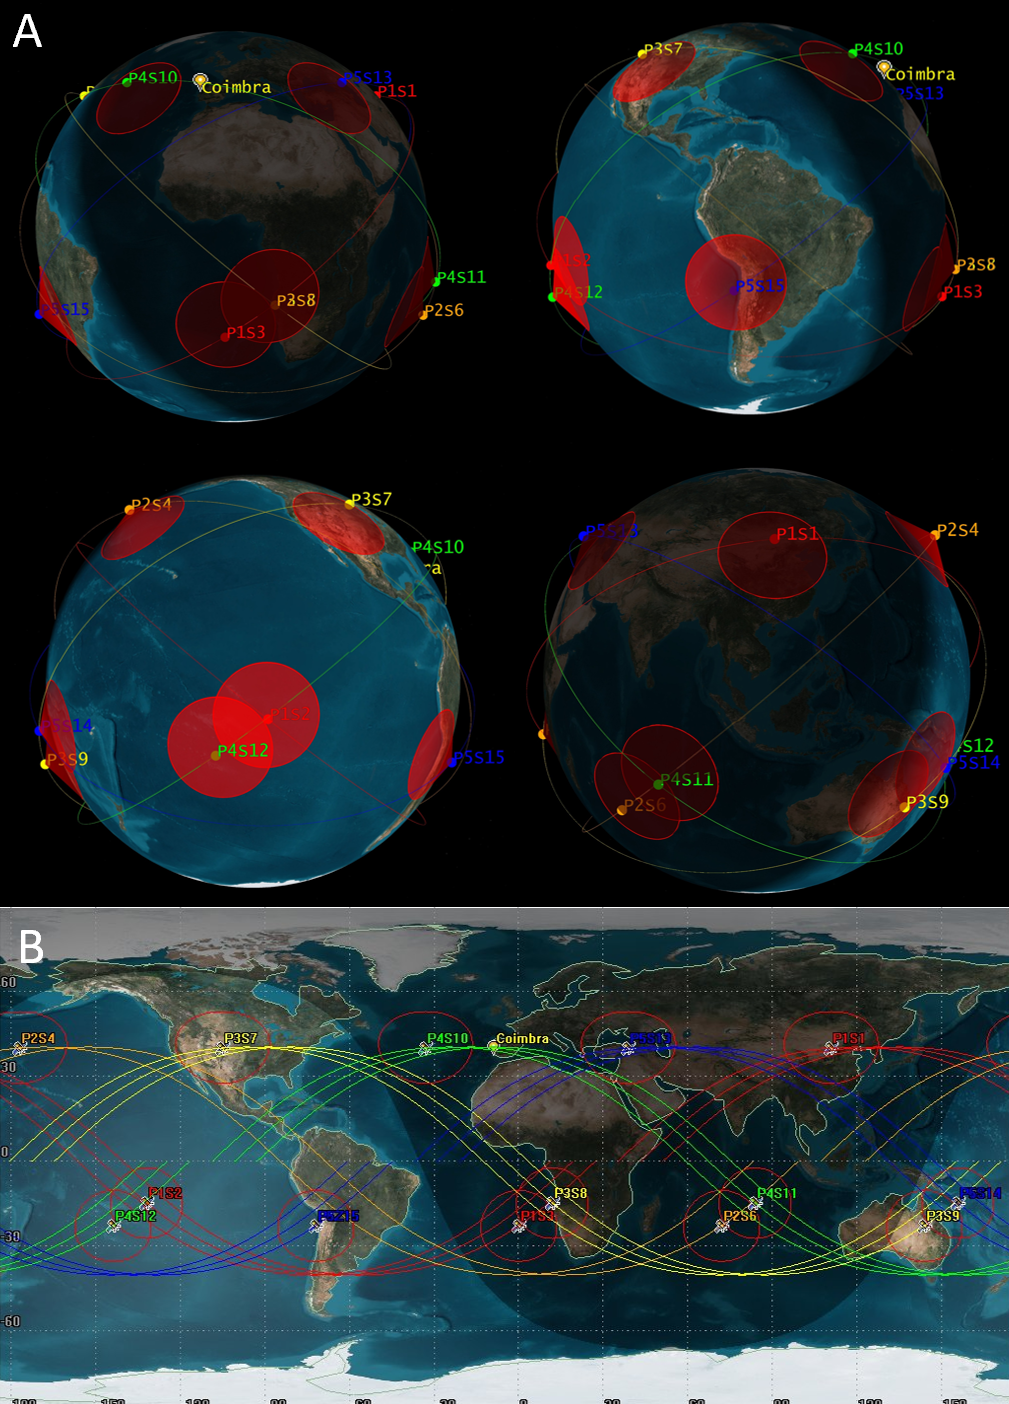
\includegraphics[width=0.92\linewidth]{images/GaiaFireeyes_Constellation3.png}
    \caption{\footnotesize{$\mathcal{C}_{\text{Zoom}} = \mathcal{C}_{15/5/72}$ constellation geometry. \textbf{(a)}~Four 3D views of the orbital configuration, showing the 15 satellites distributed across 5 planes (3 satellites per plane). \textbf{(b)}~Ground track plot over the global map. Each orbital plane is colour-coded: Plane~1 (P1)~-- red; Plane~2 (P2)~-- orange; Plane~3 (P3)~-- yellow; Plane~4 (P4)~-- green; Plane~5 (P5)~-- blue. The spacecraft conical sensor envelopes visible in the panels represent the maximum geometrical observation-link access at off-nadir angle $\eta_{\max} = 65^{\circ}$; they represent the space-segment access geometry.}}
    \label{fig:GaiaFireeyes_Constellation3}
\end{figure}




\section{Zoom Layer Results and Performance Analysis}
\label{sec:zoom_layer}

The goal of this section is to analyze the performance of the $\mathcal{C}_{\text{Zoom}}$ constellation if the sensor effective field of view $\eta$ is a variable. We want to define a set of $\eta$ values to explore this metrics results. 

As described in Section~\ref{sec:constellation_plane1}, the temporal resolution of the constellation $t_{\text{revisit}}$ is determined by the number of spacecrafts per plane $N_{\text{s/P}} = 3$. To achieve a full day coverage, this same setting of spacecraft need to be copied into new planes sharing the same origin but with a Right Ascension of the Ascending Node (RAAN) phase angle $\Omega$ between the planes. The number of orbital planes $P$ required to maintain $t_{\text{revisit}} \approx 30$\,min for a full day, is set by the effective observation-link sequence time $\tau_{\text{seq,eff}}$, i.e.\ the duration off the pass sequences of the 3 coplanar satellites over the core domain $\mathcal{D}_{\text{core}}$. Given a full day $t_{\text{day}} = 1440$\,min, the minimum plane P count is:
\begin{equation}
    P = \frac{t_{\text{day}}}{\tau_{\text{seq,eff}}}
    \label{eq:planes_from_tau}
\end{equation}
The total satellite count follows as $T = P \times N_{\text{s/P}}$, with $N_{\text{s/P}} = 3$ fixed throughout. Because $\tau_{\text{seq,eff}}$ decreases with the maximum allowed off-nadir angle $\eta$, a sensor restricted to small $\eta$ values forces a proportionally larger constellation. Table~\ref{tab:zoom_layer_configurations} and Figure~\ref{fig:observation_link_VS_eta_trade_off} quantify this trade-off across four representative configurations. Configuration ~\# c1 ($\eta = 65^{\circ}$) yields the minimum viable constellation of $T = 15$ satellites and is the selected $\mathcal{C}_{\text{Zoom}}$ baseline, conditional on a sensor with sufficient effective FOV (via tactical pointing or scanning) to exploit $\eta_{\max} \approx 65^{\circ}$.

\begin{table}[H]
    \centering
    \caption{\footnotesize{Off-nadir angle $\eta$ vs.\ constellation size trade-off (Eq.~\ref{eq:planes_from_tau}, $t_{\text{day}} = 1440$\,min, $N_{\text{s/P}} = 3$). Baseline configuration highlighted.}}
    \label{tab:zoom_layer_configurations}
    \small
    \begin{tabular}{cccccc}
        \toprule
        \textbf{c\#} & 
        \textbf{Off-Nadir $\boldsymbol{\eta}$ [\textdegree]} & 
        \textbf{$\boldsymbol{\tau_{\text{seq,eff}}}$ [min]} & 
        \textbf{$\boldsymbol{P}$ [planes]} & 
        \textbf{Sat/P} &
        \textbf{Total Sats $\boldsymbol{T}$} \\
        \midrule
        \rowcolor{green!15}
        1 & $65$ & $297.0$  & $5$  & $3$ & $\mathbf{15}$ \\
        2 & $45$          & $238.4$  & $7$  & $3$ & $21$          \\
        3 & $30$          & $172.41$ & $9$  & $3$ & $27$          \\
        4 & $15$          & $106.7$  & $14$ & $3$ & $\mathbf{42}$ \\
        \bottomrule
    \end{tabular}
    \label{tab:Czoom_eta_configurations}
\end{table}

The $\mathcal{C}_{\text{Zoom}}$ is subsequently analyzed for the metrics: Average Pass Duration; Number of Pass; Temporal Coverage. These performances are evaluated over the global domain $\mathcal{D}_{\text{global}}$ against fire-prone regions~(FPR) grouped by recurrence: recurrent ($r$, ${>}7$ fires/decade), occasional ($o$, ${<}3$), and infrequent ($i$, ${<}1$). The following subsections focus on the highest-priority recurrent group~$\mathrm{FPR}_{r}$.

\begin{figure}[H]
    \centering
    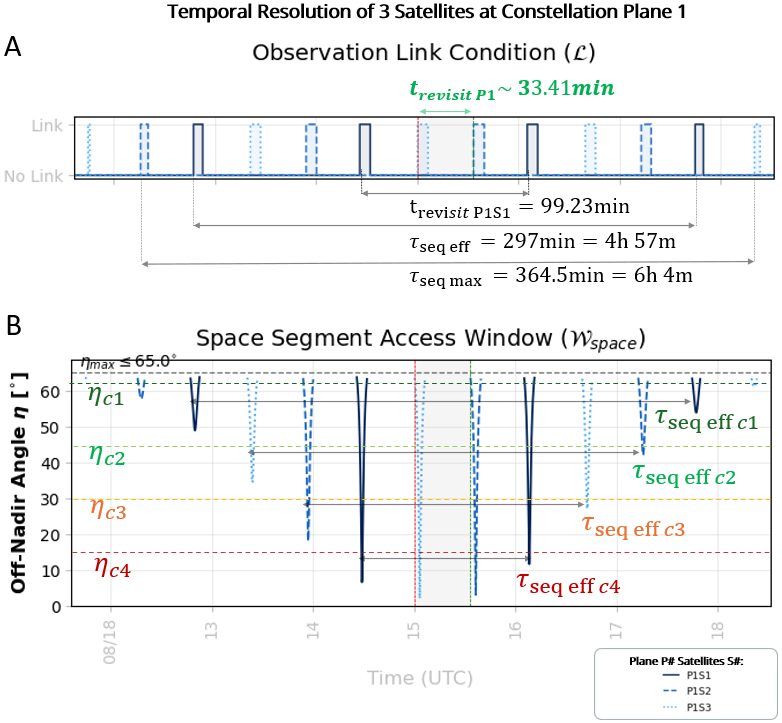
\includegraphics[width=0.82\linewidth]{images/observation_link_VS_eta_trade_off.png}
    \caption{\footnotesize{Zoom layer sensor trade-off analysis. (A) Observation link condition and temporal resolution analysis for a single plane. (B) Space segment access window ($\mathcal{W}_{\text{space}}$) as a function of off-nadir angle $\eta$. A wider allowable angle (e.g., $\eta_{c1}$) yields a longer effective sequence $\tau_{\text{seq, eff}}$, reducing the number of planes needed.}}
    \label{fig:observation_link_VS_eta_trade_off}
\end{figure}


%%% ================================================================
%%% Phase 1 — Performance Metrics Definition
%%% ================================================================
\subsection{Performance Metrics Definition}
\label{sec:performance_metrics_definition}

Before presenting the simulation results, this subsection defines the performance metrics used throughout this analysis.  All quantities are evaluated over a single-day simulation window ($t_{\text{day}} = 1440$\,min) and are computed per ground-grid points $P_j$ (120x360 grid cells) unless otherwise noted.

\begin{enumerate}
    \item \textbf{Off-nadir angle} ($\eta$): the angle between the satellite nadir direction and the line of sight to a ground  defined at equation \ref{eq:eta} and with values cited in Figure \ref{fig:observation_link_VS_eta_trade_off}

    \item \textbf{Number of passes} ($N_{\text{pass}}$): the total count of individual satellite passes per day over a given ground point $P_j$, where a pass is an uninterrupted interval during which the observation-link condition (Eq.~\ref{eq:observation_link_condition}) is satisfied.

    \item \textbf{Average pass duration} ($\bar{t}_{\text{pass}}$): the mean duration of a single pass over $P_j$, in minutes. It represents the mean imaging dwell time available to the payload per overpass event.

    \item \textbf{Temporal coverage} ($T_{\text{cov}}$): the cumulative time (hours per day) during which spacecrafts of the constellation satisfies the observation-link condition over a ground point $P_j$.
    \item \textbf{Minimum revisit time} ($\Delta t_{\min}$): the shortest gap between two consecutive passes over a ground point $P_j$, typically arising from the overlap between the last satellites of one orbital plane sequence and the first satellites of the next (see Fig.~\ref{fig:obs_links_5planes} for a visual example at Coimbra).

    \item \textbf{Maximum revisit time} ($\Delta t_{\max}$): the longest gap between consecutive passes over $P_j$. For the $\mathcal{C}_{\text{Zoom}}$ baseline design, this value is driven by the inter-plane RAAN spacing and the design target of $\Delta t_{\max} = t_{\text{revisit}} \approx 30$\,min.

    \item \textbf{Average revisit time} ($\Delta t_{\text{avg}}$): the mean temporal gap between consecutive passes over $P_j$, averaged over all gaps in the day.
\end{enumerate}

The analysis proceeds in four stages.  First, the global-domain maps of geometric and pass metrics ($\eta$, $N_{\text{pass}}$, $\bar{t}_{\text{pass}}$) are presented to characterize the observation geometry quality of the constellation (Section~\ref{sec:global_geometric_pass_metrics}).  Second, the temporal revisit metrics ($\Delta t_{\min}$, $\Delta t_{\text{avg}}$, $\Delta t_{\max}$) are mapped over $\mathcal{D}_{\text{global}}$ (Section~\ref{sec:global_temporal_metrics_Vs_eta}).  Third, the temporal coverage $T_{\text{cov}}$ is analyzed globally and then filtered through fire-prone region masks (Section~\ref{sec:global_Domain_temporal_coverage_Vs_eta}).  Finally, the metrics are extracted at the latitude of the core domain $\mathcal{D}_{\text{core}}$ to quantify the constellation performance over Portugal (Section~\ref{sec:portugal_core_domain_metrics_derive_from_global_domain_results}).


%%% ================================================================
%%% Phase 2 — Global Domain Geometric and Pass Metrics
%%% ================================================================
\subsection{Global Domain Geometric and Pass Metrics}
\label{sec:global_geometric_pass_metrics}

Figures~\ref{fig:c_zoom_avg_off_nadir}--\ref{fig:C_zoom_global_average_pass} map the three geometric and pass metrics $(\bar{\eta}$, $N_{\text{pass}}$, and $\bar{t}_{\text{pass}})$ over $\mathcal{D}_{\text{global}}$ for the four $\eta$ configurations of Table~\ref{tab:zoom_layer_configurations}.

The average off-nadir angle map (Fig.~\ref{fig:c_zoom_avg_off_nadir}) reveals that the latitude band $\phi \approx \pm\,40^{\circ}$ have the lowest $\bar{\eta} \approx 50^{\circ}$, meaning that satellites overpass this region closest to the nadir direction of the local grid points~$P_j(\phi \approx \pm\,40^{\circ})$.  This is a direct consequence of the RGTO inclination ($i = 40.02^{\circ}$): the ground-track density peaks near the orbital turning latitudes, concentrating low effective field of view passes over this band.  Outside $\phi \approx \pm\,40^{\circ}$, $\bar{\eta}$ rises to a near-uniform plateau of $\sim\!54$--$55^{\circ}$ across the remaining latitudes.  Crucially, the $\phi \approx 40^{\circ}$\,N belt coincides with both the core domain~$\mathcal{D}_{\text{core}}$ and the temperate-forest recurrent fire-prone regions (Fig.~\ref{fig:c_zoom_global_FRP_recurrent_ocasional_Tcoverage_eta63}), confirming that the orbit design concentrates the best observation geometry over the regions of highest mission priority.

The number-of-passes map (Fig.~\ref{fig:C_zoom_global_number_passes}) shows that the latitude of maximum $N_{\text{pass}}$ is displaced slightly equator-ward from $\phi = \pm\,40^{\circ}$, peaking near $\phi \approx \pm\,30^{\circ}$.  This offset arises because sub-satellite tracks from adjacent orbital planes converge and overlap at latitudes below the turning point, compounding the pass count.  The $\phi \approx \pm\,30^{\circ}$ overlap band may represent a favourable communication intercept latitude for a future inter-layer relay link between the Zoom layer and a communication layer $\mathcal{C}_{\text{Comm}}$, \inlineReq{R36}.

Finally, the average pass duration map (Fig.~\ref{fig:C_zoom_global_average_pass}) mirrors the $\bar{\eta}$ pattern: $\bar{t}_{\text{pass}}$ reaches its maximum of $\sim\!6$\,min at $\phi \approx \pm\,40^{\circ}$, where the near-nadir geometry prolongs each overpass, while the global background settles at $\sim\!5$\,min.  Together, the low $\bar{\eta}$ and high $\bar{t}_{\text{pass}}$ at the core-domain latitude confirm that $\mathcal{C}_{\text{Zoom}}$ delivers both the best image quality and the longest dwell time over $\mathcal{D}_{\text{core}}$. A result that will be corroborated by the global Fire Prone Regions coverage statistics in Section~\ref{sec:global_Domain_fire_prone_regions_statistics}.

\begin{figure}[H]
    \centering
    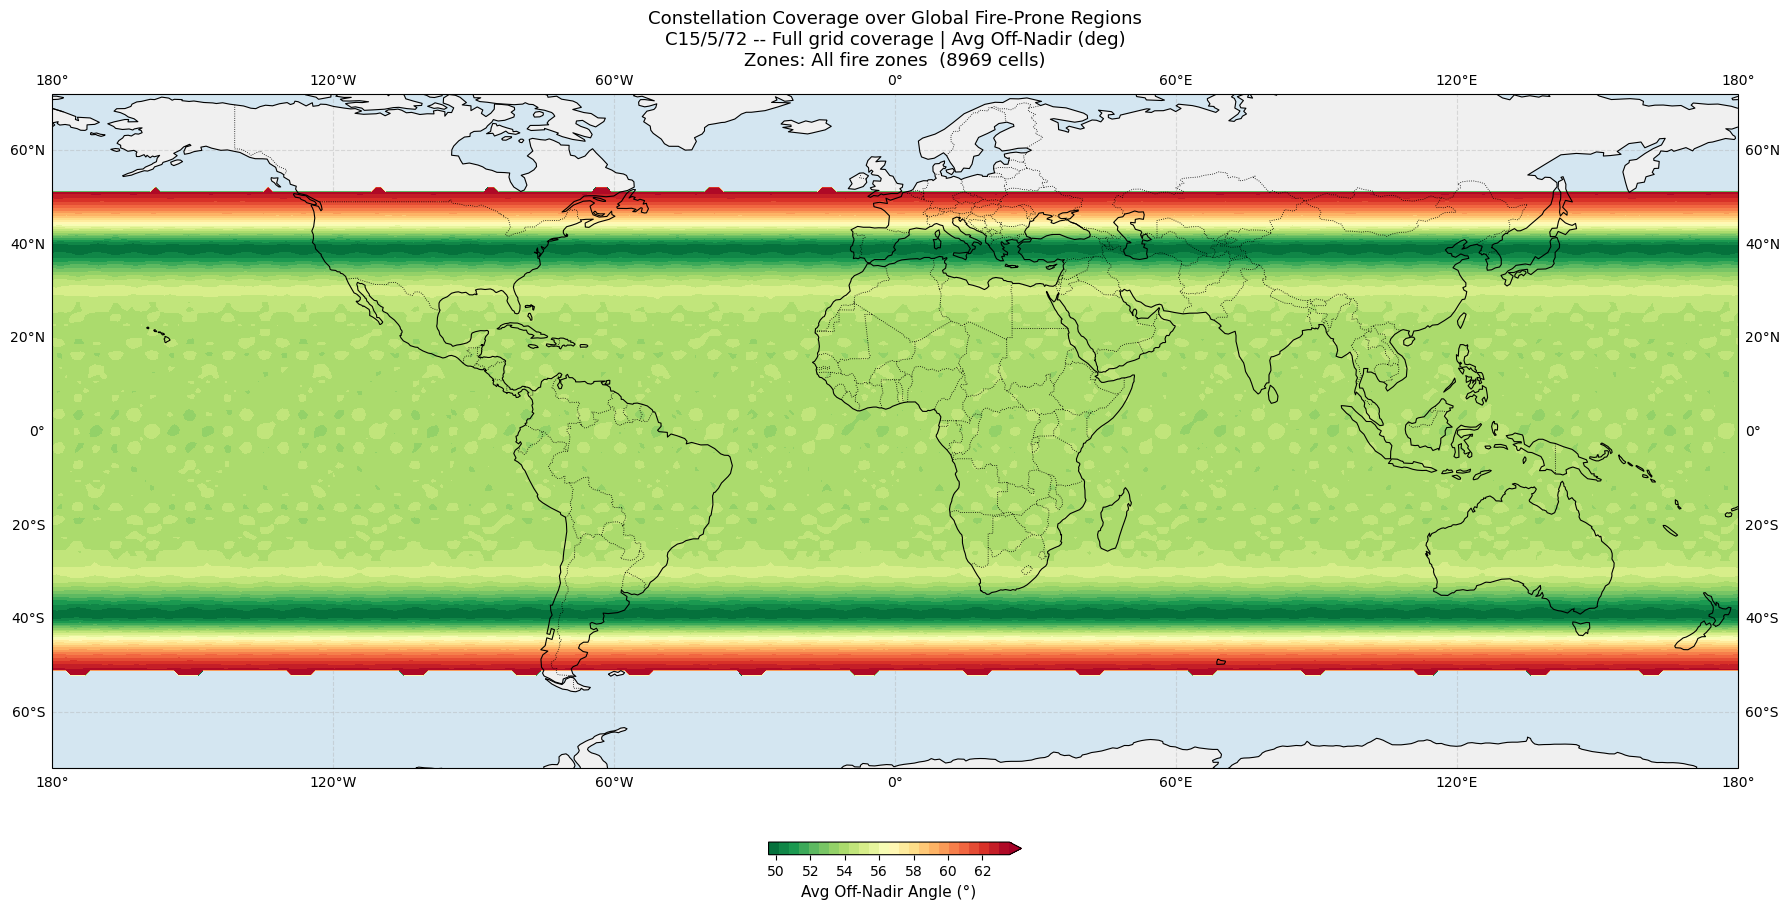
\includegraphics[width=1\linewidth]{images/c_zoom_avg_off_nadir.png}
    \caption{\footnotesize{Global map of the average off-nadir angle~$\bar{\eta}$ for $\mathcal{C}_{\text{Zoom}}$ across the four $\eta$ configurations (Table~\ref{tab:zoom_layer_configurations}).  The minimum $\bar{\eta} \approx 50^{\circ}$ occurs at latitudes $\phi \approx \pm\,40^{\circ}$, coinciding with $\mathcal{D}_{\text{core}}$ and the recurrent temperate Fire Prone Regions belt, while a near-uniform plateau of $\sim\!55^{\circ}$ covers the remaining latitudes.}}
    \label{fig:c_zoom_avg_off_nadir}
\end{figure}

\begin{figure}[H]
    \centering
    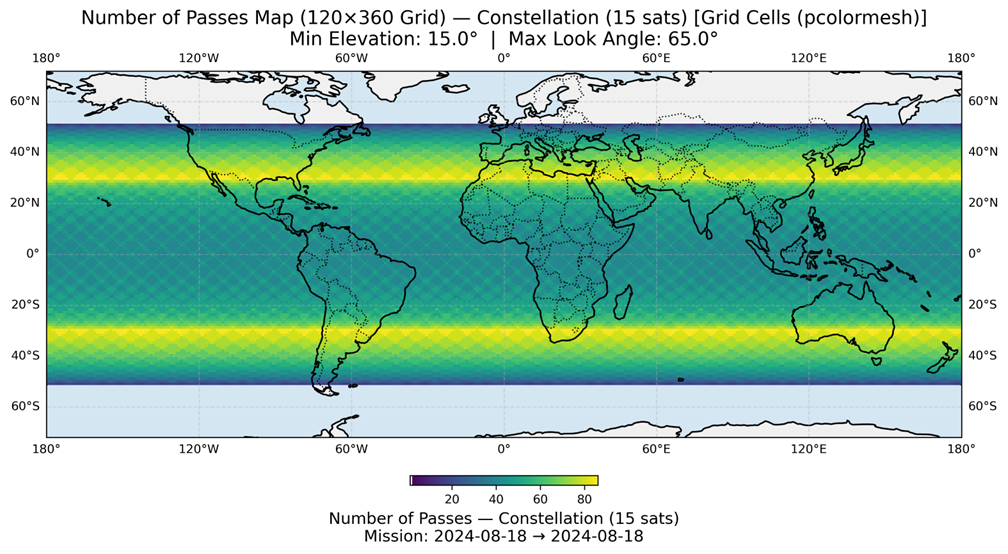
\includegraphics[width=1\linewidth]{images/C_zoom_global_number_passes.png}
    \caption{\footnotesize{Global map of the number of passes per day~$N_{\text{pass}}$ for $\mathcal{C}_{\text{Zoom}}$.  The maximum $N_{\text{pass} = 80}$ peaks near $\phi \approx \pm\,30^{\circ}$ due to inter-plane ground-track overlap, slightly equator-ward of the optimal geometry latitude, creating an optimal communication region.}}
    \label{fig:C_zoom_global_number_passes}
\end{figure}

\begin{figure}[H]
    \centering
    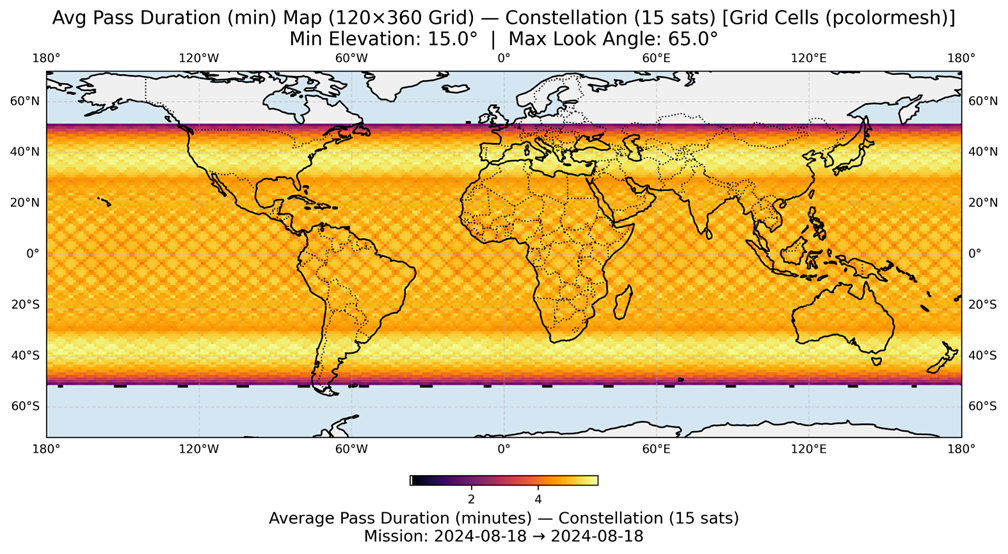
\includegraphics[width=1\linewidth]{images/C_zoom_global_average_pass.png}
    \caption{\footnotesize{Global map of the average pass duration~$\bar{t}_{\text{pass}}$ for $\mathcal{C}_{\text{Zoom}}$.  The maximum dwell of $\sim\!6$\,min is reached at $\phi \approx \pm\,40^{\circ}$ (RGTO resonance latitude), while the global average is $\sim\!5$\,min.}}
    \label{fig:C_zoom_global_average_pass}
\end{figure}


%%% ================================================================
%%% Phase 3 — Global Domain Temporal Metrics (Revisit)
%%% ================================================================
\subsection{Global Domain Temporal Metrics}
\label{sec:global_temporal_metrics_Vs_eta}

Figures~\ref{fig:c_zoom_min_revisit}--\ref{fig:c_zoom_max_revisit} map the three revisit metrics $(\Delta t_{\min}$, $\Delta t_{\text{avg}}$, and $\Delta t_{\max})$ over $\mathcal{D}_{\text{global}}$ for the baseline $\mathcal{C}_{\text{Zoom}}$ $\eta = 65^{\circ}$ configuration.

The minimum revisit map (Fig.~\ref{fig:c_zoom_min_revisit}) shows that the latitude band $\phi \approx \pm\,[25^{\circ}$--$45^{\circ}]$ achieves the most uniform $\Delta t_{\min} \approx 25$\,min, reflecting the dense plane-overlap geometry identified in Section~\ref{sec:global_geometric_pass_metrics}.  Gaps of higher $\Delta t_{\min}$ appear between $\phi \approx 0^{\circ}$--$20^{\circ}$, where the inter-plane phasing produces localized coverage holes of $\Delta t_{\min}$ 30min revisit surrounded by 10 min revisit regions.

The maximum revisit map (Fig.~\ref{fig:c_zoom_max_revisit}) confirms that across the same mid-latitude belt ($\phi \approx \pm\,[20^{\circ}$--$40^{\circ}]$) $\Delta t_{\max}$ remains close to the design target of $\sim\!30$\,min.  Near the equator, however, a gap band around $\phi \approx \pm\,15^{\circ}$ drives $\Delta t_{\max}$ up to $\sim\!115$\,min, corresponding to an period of the day with a temporal gap where no satellite satisfies the observation-link condition for approximately two hours.

The average revisit map (Fig.~\ref{fig:c_zoom_avg_revisit}) reaches its worst result at $\phi \approx \pm\,15^{\circ}$at with $\Delta t_{\text{avg}} \approx 50$\,min, and optimum values of $\Delta t_{\text{avg}} \approx 25$\,min near $\phi \approx \pm\,30^{\circ}$, the same pass-count peak latitude at Figure \ref{fig:C_zoom_global_number_passes}.  However, as established in Section~\ref{sec:global_geometric_pass_metrics}, this latitude does not coincide with the best observation geometry ($\bar{\eta}$ minimum at $\phi \approx \pm\,40^{\circ}$), making it more suited to a communication relay function than to high-resolution imaging.  At the core-domain latitude ($\phi \approx 40^{\circ}$\,N), $\Delta t_{\text{avg}} \approx 30$\,min, matching the mission design requirement $t_{\text{revisit}} \approx 30$\,min and confirming that $\mathcal{C}_{\text{Zoom}}$ delivers the specified monitoring cadence over Portugal $\mathcal{D}_{\text{Core}}$the recurrent temperate fire-prone regions.

\begin{figure}[H]
    \centering
    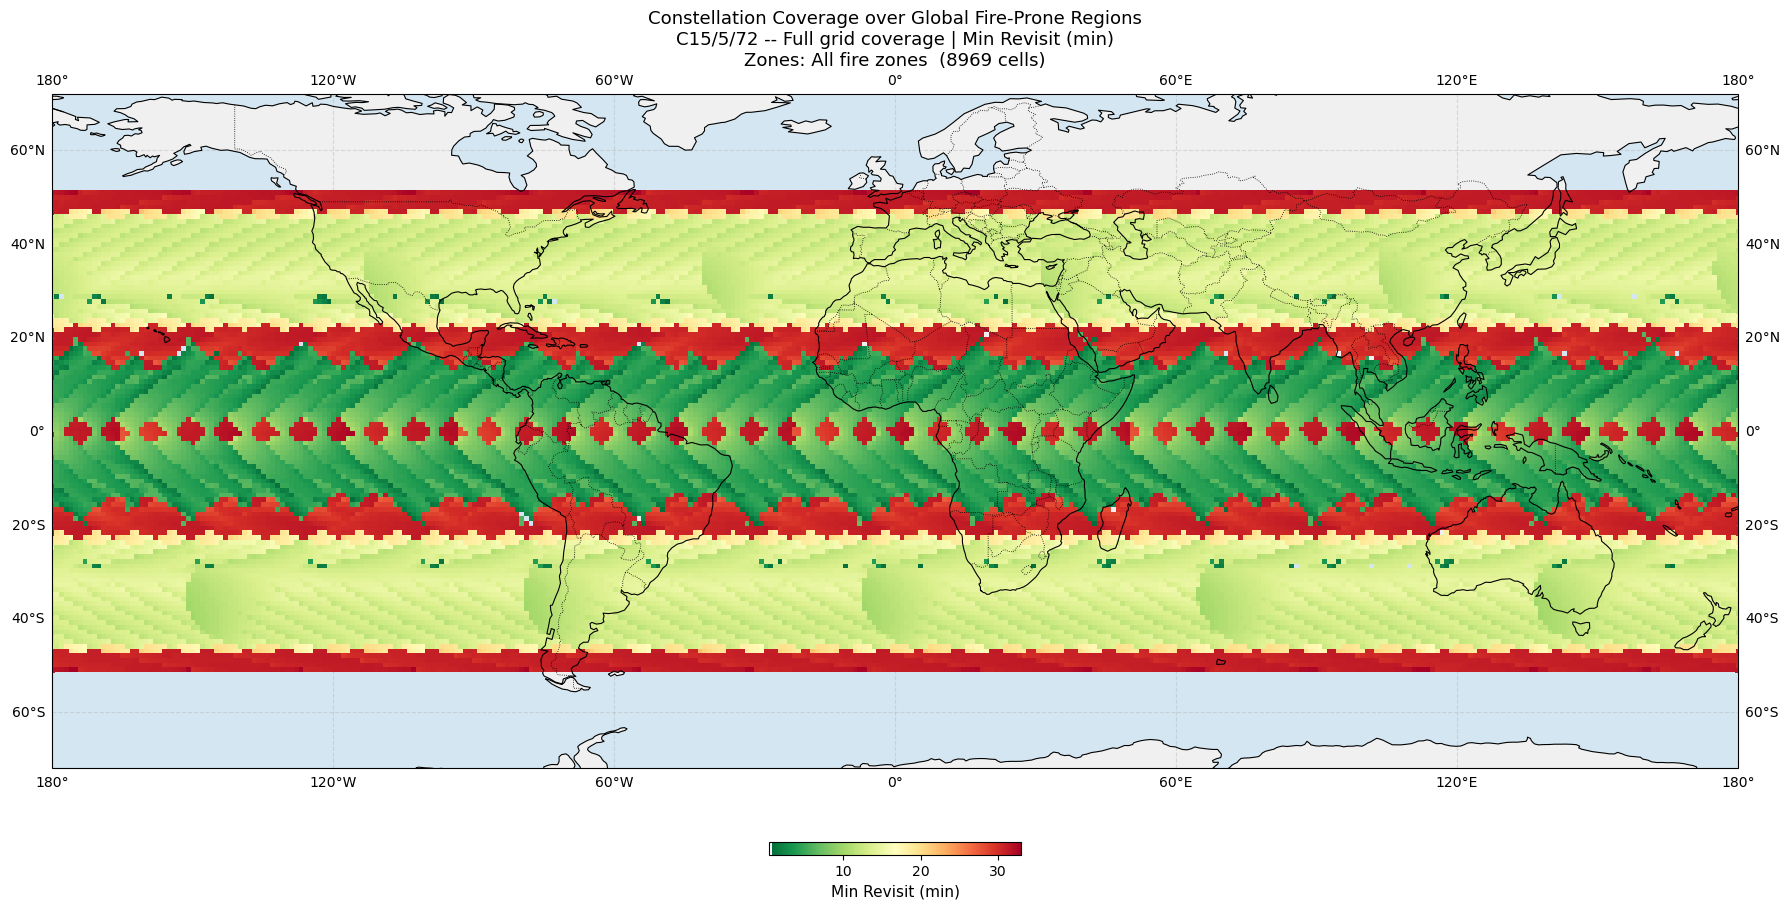
\includegraphics[width=1\linewidth]{images/c_zoom_min_revisit.png}
    \caption{\footnotesize{Global map of the minimum revisit time~$\Delta t_{\min}$ for $\mathcal{C}_{\text{Zoom}}$ ($\eta = 65^{\circ}$).  The most uniform band ($\Delta t_{\min} \approx 25$\,min) spans $\phi \approx \pm\,25^{\circ}$--$45^{\circ}$; sporadic gaps near the equator reflect inter-plane phasing discontinuities.}}
    \label{fig:c_zoom_min_revisit}
\end{figure}

\begin{figure}[H]
    \centering
    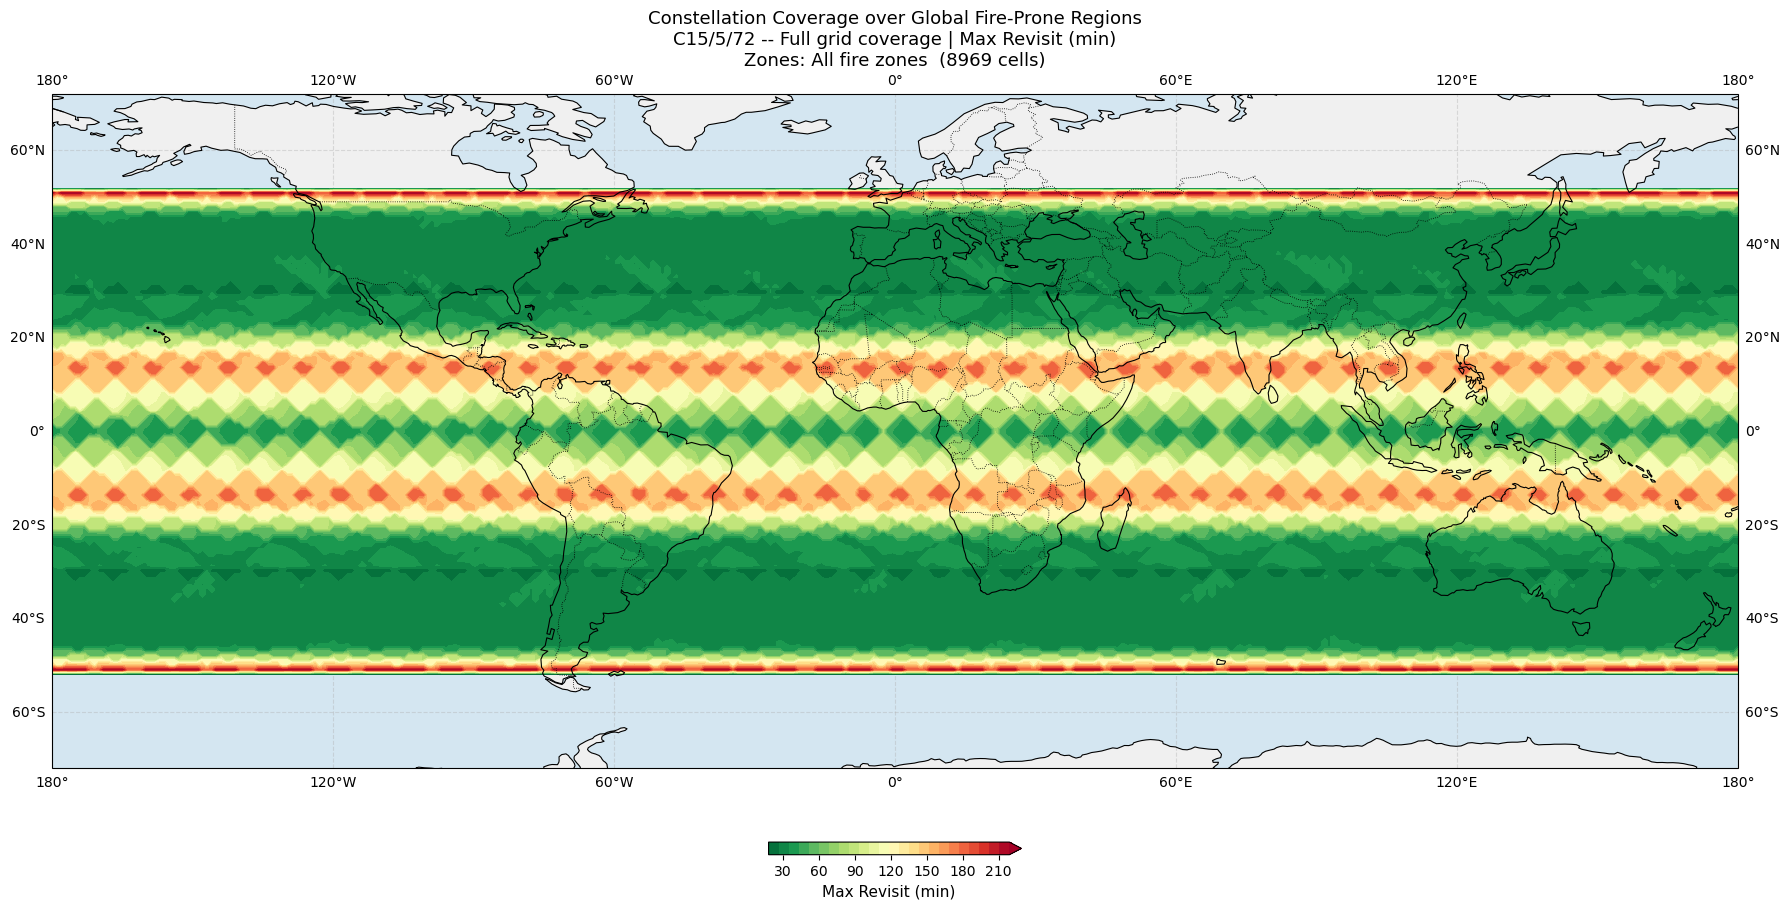
\includegraphics[width=1\linewidth]{images/c_zoom_max_revisit.png}
    \caption{\footnotesize{Global map of the maximum revisit time~$\Delta t_{\max}$ for $\mathcal{C}_{\text{Zoom}}$ ($\eta = 65^{\circ}$).  Mid-latitudes maintain $\Delta t_{\max} \approx 30$\,min; the worst-case gap of $\sim\!115$\,min appears near $\phi \approx \pm\,15^{\circ}$ due to an inter-plane RAAN discontinuity.}}
    \label{fig:c_zoom_max_revisit}
\end{figure}

\begin{figure}[H]
    \centering
    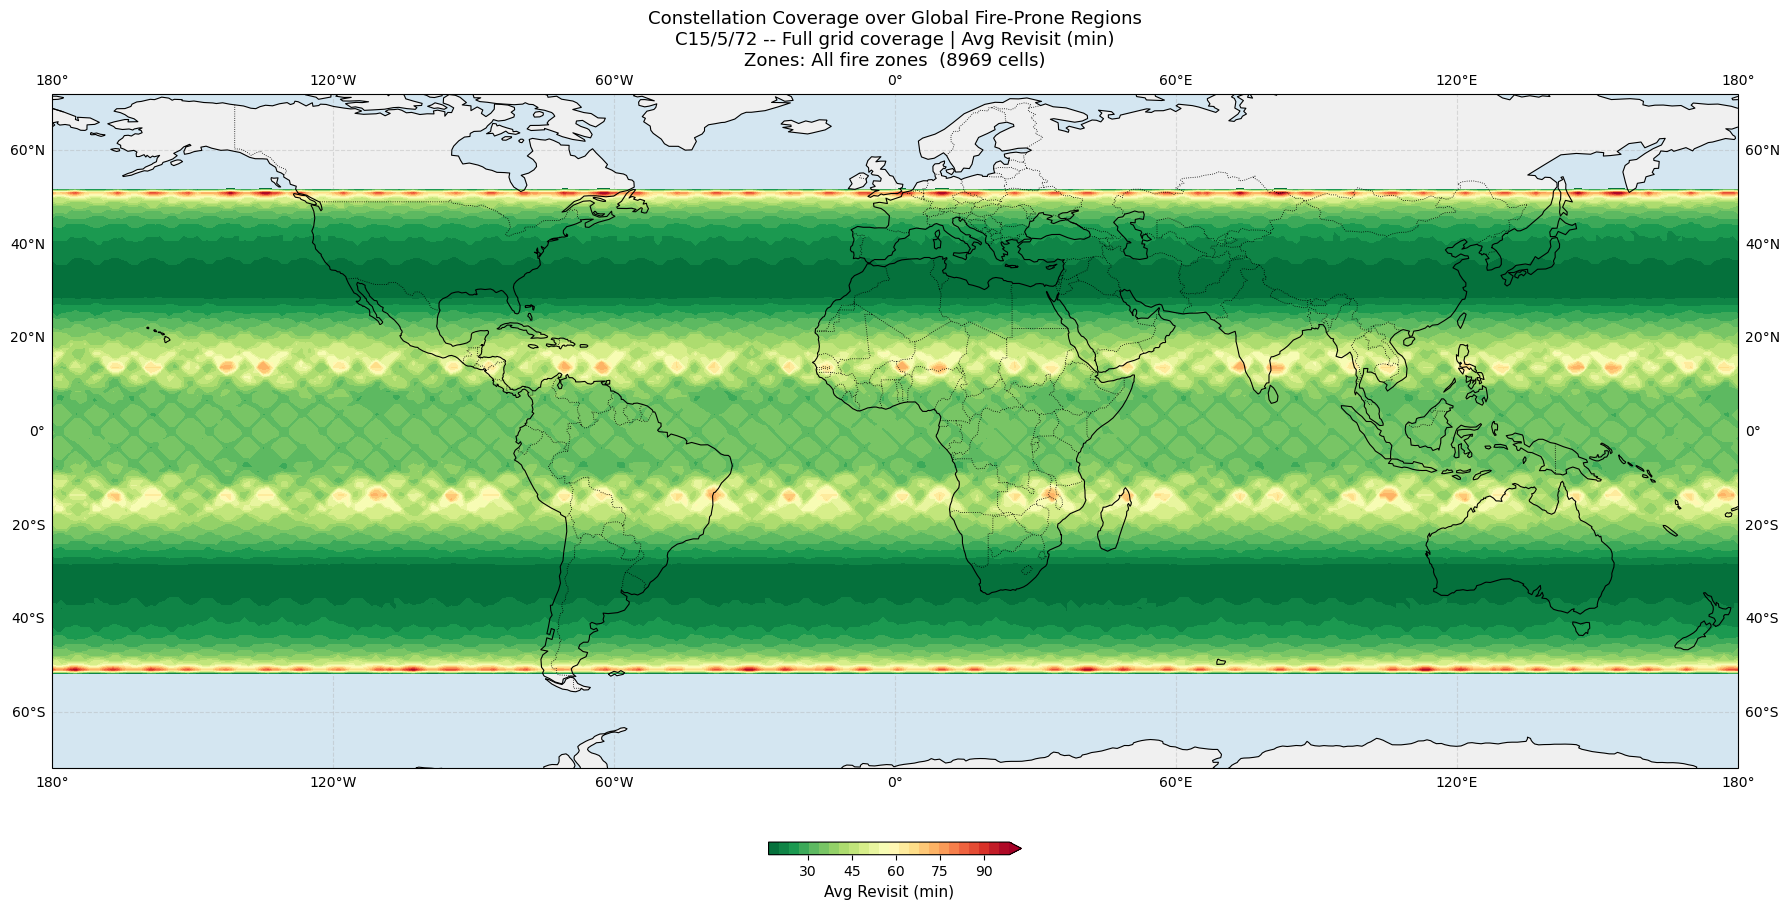
\includegraphics[width=1\linewidth]{images/c_zoom_avg_revisit.png}
    \caption{\footnotesize{Global map of the average revisit time~$\Delta t_{\text{avg}}$ for $\mathcal{C}_{\text{Zoom}}$ ($\eta = 65^{\circ}$).  The optimum $\Delta t_{\text{avg}} \approx 25$\,min occurs near $\phi \approx \pm\,30^{\circ}$ (pass-count peak); at the core-domain latitude $\Delta t_{\text{avg}} \approx 30$\,min, satisfying the design target.}}
    \label{fig:c_zoom_avg_revisit}
\end{figure}




%%% ================================================================
%%% Phase 4 — Global Temporal Coverage vs. Off-Nadir Angle
%%% ================================================================
\subsection{Global Domain Temporal Coverage Vs.\ Off-Nadir Angle}
\label{sec:global_Domain_temporal_coverage_Vs_eta}

Figure~\ref{fig:c_zoom_global_Tcovera_eta63} maps the temporal coverage~$T_{\text{cov}}$ over $\mathcal{D}_{\text{global}}$ for the baseline $\mathcal{C}_{\text{Zoom}}$ $\eta = 65^{\circ}$ configuration.  The latitude band $\phi \approx \pm\,30^{\circ}$ have the highest $T_{\text{cov}} \approx 7$\,h/day, a region suited for inter-layer communication relay already identified as the pass-count and revisit-time optimum (Sections~\ref{sec:global_geometric_pass_metrics}--\ref{sec:global_temporal_metrics_Vs_eta}).  At the core-domain latitude ($\phi \approx 40^{\circ}$\,N), $T_{\text{cov}} \approx 6$\,h/day; more broadly, the band $\phi \approx \pm\,[30^{\circ}$--$45^{\circ}]$ sustains $T_{\text{cov}} \approx 6$--$7$\,h/day, coinciding with the temperate fire-prone regions where high-cadence monitoring is most needed.  Equatorial latitudes ($|\phi| < 30^{\circ}$) reach $T_{\text{cov}} \approx 4$\,h/day, providing coverage for tropical fire-prone biomes.

The appendix maps (Figs.~\ref{fig:c_zoom_global_Tcoverage_eta45}--\ref{fig:c_zoom_global_Tcoverage_eta15}) illustrate the impact of reducing $\eta$.  At $\eta = 45^{\circ}$, the mid-latitude coverage contracts but still envelops $\mathcal{D}_{\text{core}}$; at $\eta = 30^{\circ}$, coverage fill Portugal area $\phi \approx 40^{\circ}$\,N; and at $\eta = 15^{\circ}$, only roughly half of Portugal remains within the coverage footprint.  Moreover, achieving full-day temporal resolution at lower $\eta$ demands a substantially larger constellation (e.g.\ $T = 27$ satellites in 9~planes for $\eta = 30^{\circ}$, Table~\ref{tab:zoom_layer_configurations}), increasing launch and orbital-insertion costs.  These results confirm that an effective off-nadir capability of $\eta \approx 65^{\circ}$ is a mission-critical requirement, to be addressed in future instrument-level studies through tactical pointing, scanning, or wide-swath sensor design,\inlineReq{R36}. 

\begin{figure}[H]
    \centering
    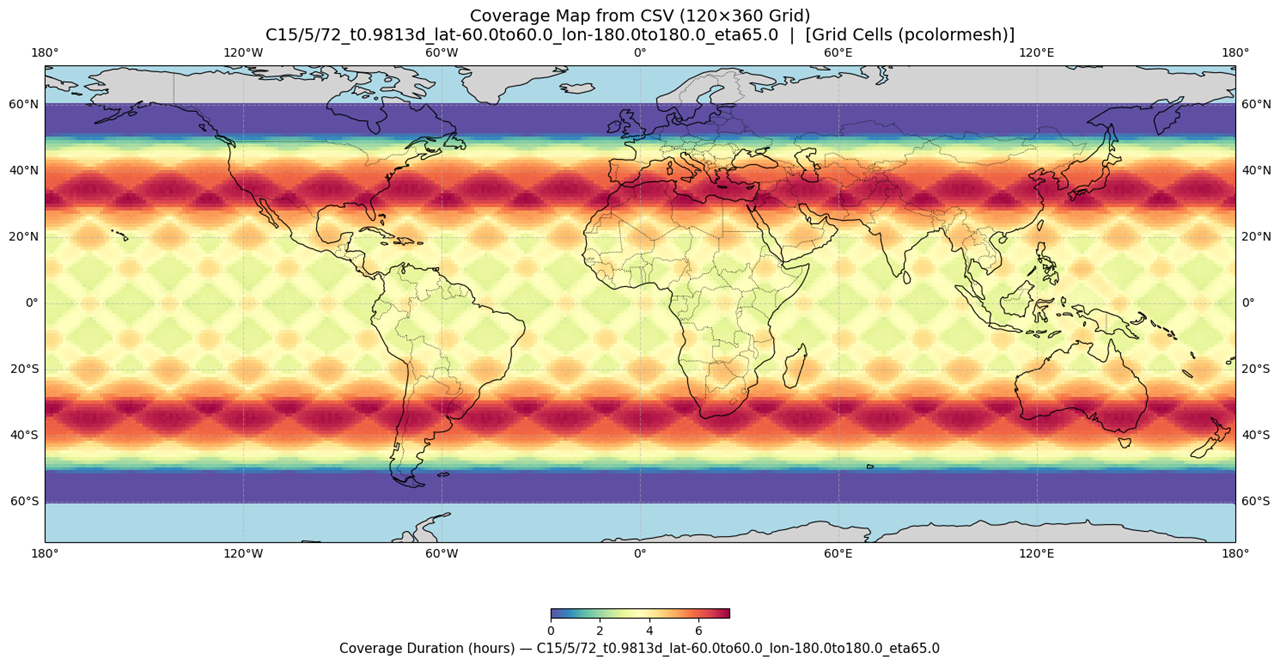
\includegraphics[width=1\linewidth]{images/c_zoom_global_Tcovera_eta63.png}
    \caption{\footnotesize{Global temporal coverage map~$T_{\text{cov}}$ for the $\mathcal{C}_{\text{Zoom}}$ baseline ($\eta = 65^{\circ}$).  Peak $T_{\text{cov}} \approx 7$\,h/day at $\phi \approx \pm\,30^{\circ}$; $T_{\text{cov}} \approx 6$\,h/day at the core-domain latitude;  coverage of ($\sim\!4$\,h/day) in equatorial regions.}}
    \label{fig:c_zoom_global_Tcovera_eta63}
\end{figure}

The corresponding temporal coverage maps for $\eta = 45^{\circ}$, $30^{\circ}$, and $15^{\circ}$ are provided in Appendix~\ref{appendix-figures} (Figs.~\ref{fig:c_zoom_global_Tcoverage_eta45}--\ref{fig:c_zoom_global_Tcoverage_eta15}).


%%% ================================================================
%%% Phase 5 — Fire-Prone Regions Coverage Analysis
%%% ================================================================
\subsection{Fire-Prone Regions Coverage Analysis}
\label{sec:fpr_coverage_analysis}

The preceding sections characterised the $\mathcal{C}_{\text{Zoom}}$ performance over the full global domain~$\mathcal{D}_{\text{global}}$.  To assess the constellation's effectiveness where it matters most, the temporal-coverage maps are now filtered through the fire-prone region (FPR) spatial masks derived from the wildfire recurrence classification introduced in Section~\ref{sec:earths_frp_targets}, represented in Figure \ref{fig:c_zoom_global_Tcoverage_FRP_groups_Spatial_Mask}.  Three recurrence groups are considered: \emph{recurrent} ($r$, $> 7 FPY$/decade), \emph{occasional} ($o$, $3 < FPY\text{/decade} \leq 7$), and \emph{infrequent} ($i$, $0 < FPY\text{/decade} \leq 3$).  Because the recurrent and occasional group concentrates the highest-priority wildfire monitoring targets, the analysis that follows focuses on the broadest operationally relevant mask for these regions grid points $P_j$.  All results correspond to the baseline $\eta = 65^{\circ}$ configuration; the off-nadir sweep maps ($\eta = 45^{\circ}$, $30^{\circ}$, $15^{\circ}$) for each FPR group are deferred to Appendix~\ref{appendix-figures}.



%%% 5a — FPR Spatial Masks

\begin{figure}[H]
    \centering
    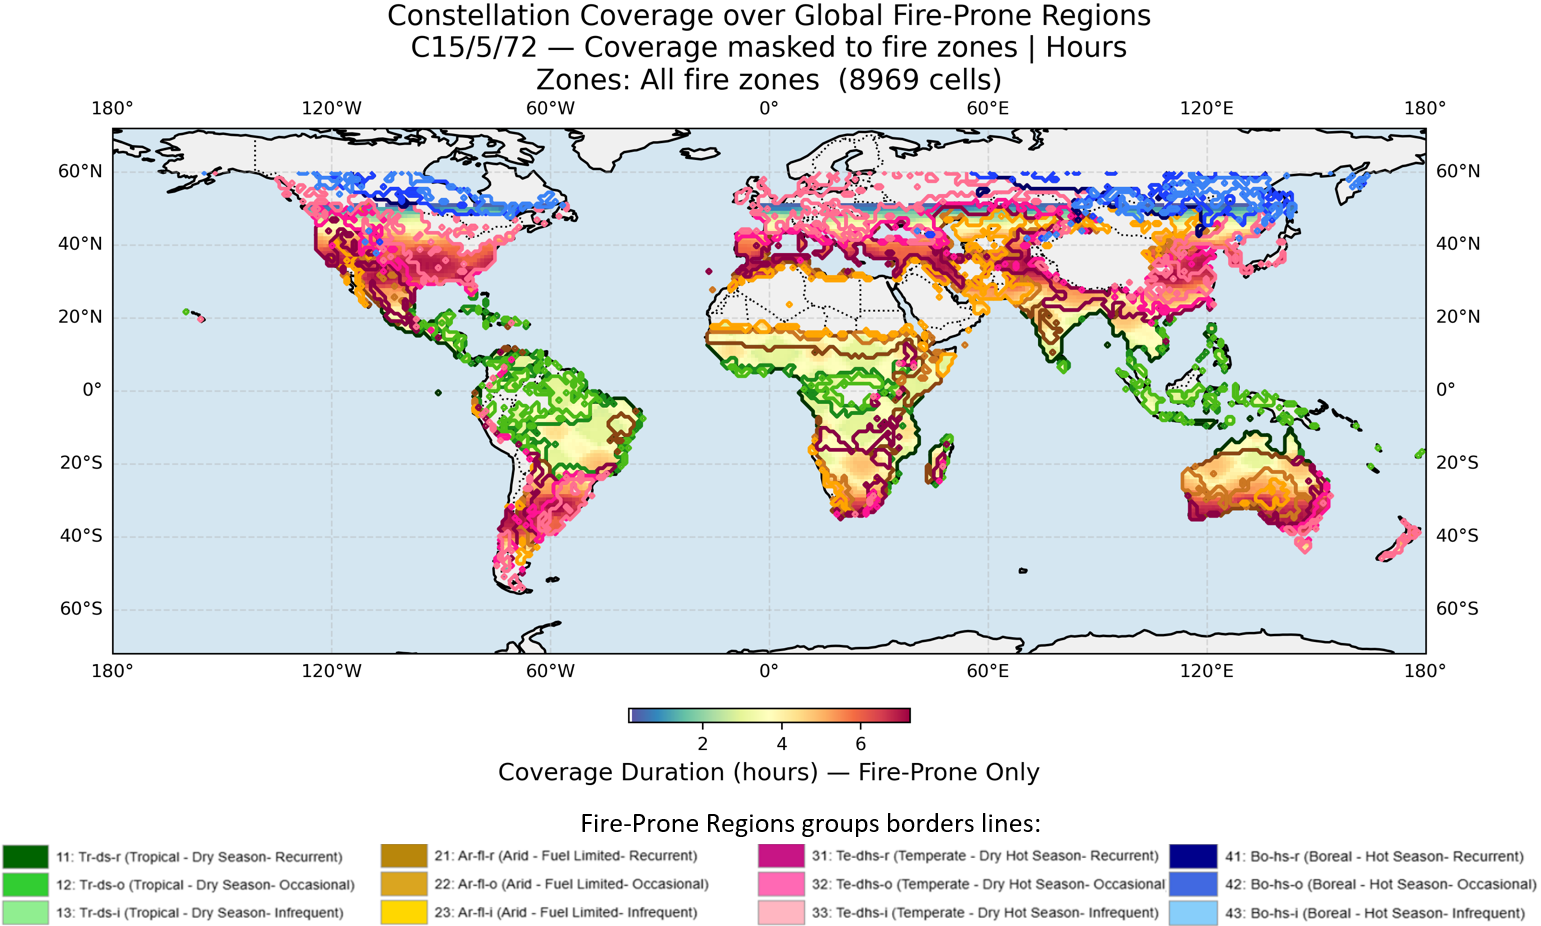
\includegraphics[width=1\linewidth]{images/c_zoom_global_Tcoverage_FRP_groups_Spatial_Mask.png}
    \caption{\footnotesize{Fire-prone region spatial masks overlaid on the $\mathcal{C}_{\text{Zoom}}$ temporal-coverage grid.  Each mask isolates the grid cells belonging to one FPR recurrence group---recurrent~($r$), occasional~($o$), and infrequent~($i$)---as classified in Section~\ref{sec:earths_frp_targets}.  The colour scale indicates $T_{\text{cov}}$ within each mask; non-FPR cells are greyed out.}}
    \label{fig:c_zoom_global_Tcoverage_FRP_groups_Spatial_Mask}
\end{figure}


%%% 5b — FPR Temporal Coverage at Baseline (η = 65°)
\subsubsection{Fire-Prone Region Temporal Coverage at Baseline ($\eta = 65^{\circ}$)}
\label{sec:fpr_temporal_coverage_baseline}

The FPR boundaries map (Fig.~\ref{fig:c_zoom_global_FRP_bondaries_Tcoverage_eta63}, Appendix~\ref{appendix-figures}) reproduces the latitude-dependent coverage pattern already identified in Section~\ref{sec:global_Domain_temporal_coverage_Vs_eta}: the highest $T_{\text{cov}}$ values concentrate at $\phi \approx \pm\,30^{\circ}$--$40^{\circ}$, coinciding with the pass-count and revisit-time optima of the constellation.  Filtering to the recurrent-only mask (Fig.~\ref{fig:c_zoom_global_FRP_recurrent_Tcoverage_eta63}, Appendix~\ref{appendix-figures}) isolates the temperate and Mediterranean forest biomes near $\phi \approx \pm\,40^{\circ}$, Tropical forests and Arid regions, confirming that constellation is optimized to the temperate biomes targets and also is great for the equatorial domains.

When the mask is broadened to include both recurrent \emph{and} occasional fire-prone regions (Fig.~\ref{fig:c_zoom_global_FRP_recurrent_ocasional_Tcoverage_eta63}), the coverage extent grows substantially: Amazonia, central Africa, south-eastern Australia, southern Africa, Chile, California, and boreal northern Europe all enter the monitored domain.  Within this combined mask, equatorial FPR zones maintain $T_{\text{cov}} > 3.5$\,h/day, while the mid-latitude temperate belt reaches $T_{\text{cov}} \approx 6$--$7$\,h/day---values consistent with the global baseline analysed in Section~\ref{sec:global_Domain_temporal_coverage_Vs_eta}.

Reading the combined FPR mask at country level reveals the breadth of the potential beneficiary nations.  In the \emph{temperate belt} ($\phi \approx \pm\,30^{\circ}$--$45^{\circ}$), where recurrent fire-prone regions concentrate and $T_{\text{cov}} \approx 5$--$7$\,h/day, the constellation covers:
\begin{itemize}[nosep]
    \item \textbf{North America}: the western and central United States (California, Oregon, Idaho, Utah, Colorado, Arizona, New~Mexico, Texas) and Mexico;
    \item \textbf{Southern Europe \& Mediterranean}: Portugal, Spain, Italy, Greece, Turkey, Morocco, Algeria, and Tunisia;
    \item \textbf{Near East \& Central Asia}: Syria, Lebanon, Iraq, Armenia, Azerbaijan, Iran, Afghanistan, Pakistan, and Uzbekistan;
    \item \textbf{South \& South-East Asia}: Nepal, northern India, Bangladesh, Myanmar, Thailand, Laos, and southern China;
    \item \textbf{Southern-hemisphere temperate}: southern Chile, Argentina, Paraguay, and Bolivia; South Africa and Madagascar; and southern and inland Australia.
\end{itemize}
In the \emph{equatorial belt} ($|\phi| < 30^{\circ}$), where $T_{\text{cov}} \approx 3$--$4$\,h/day, the constellation additionally services:
\begin{itemize}[nosep]
    \item \textbf{Caribbean \& Central America}: Cuba, Guatemala, and the remaining Central American nations;
    \item \textbf{South America}: Venezuela, the Brazilian Amazon basin, the Cerrado savanna, the Pantanal wetlands, and the semi-arid Nordeste region of Brazil;
    \item \textbf{Sub-Saharan Africa}: Africa being the most fire-active continent globally, have it's fire belt covered, including Nigeria, Congo, Angola, Mozambique, and Somalia, among others;
    \item \textbf{Maritime South-East Asia}: Indonesia and the Philippines.
\end{itemize}
Altogether, the $\mathcal{C}_{\text{Zoom}}$ constellation provides operationally useful temporal coverage to the vast majority of fire-prone nations worldwide.  The temperate-belt countries benefit from the highest $T_{\text{cov}}$ and the shortest revisit times, a direct consequence of the RGTO inclination placing the ground-track density peak at the latitudes of these regions. The equatorial nations, although receiving lower absolute $T_{\text{cov}}$, still obtain continuous daily monitoring that substantially exceeds the revisit cadence of current polar-orbiting fire-detection systems.

\begin{figure}[H]
    \centering
    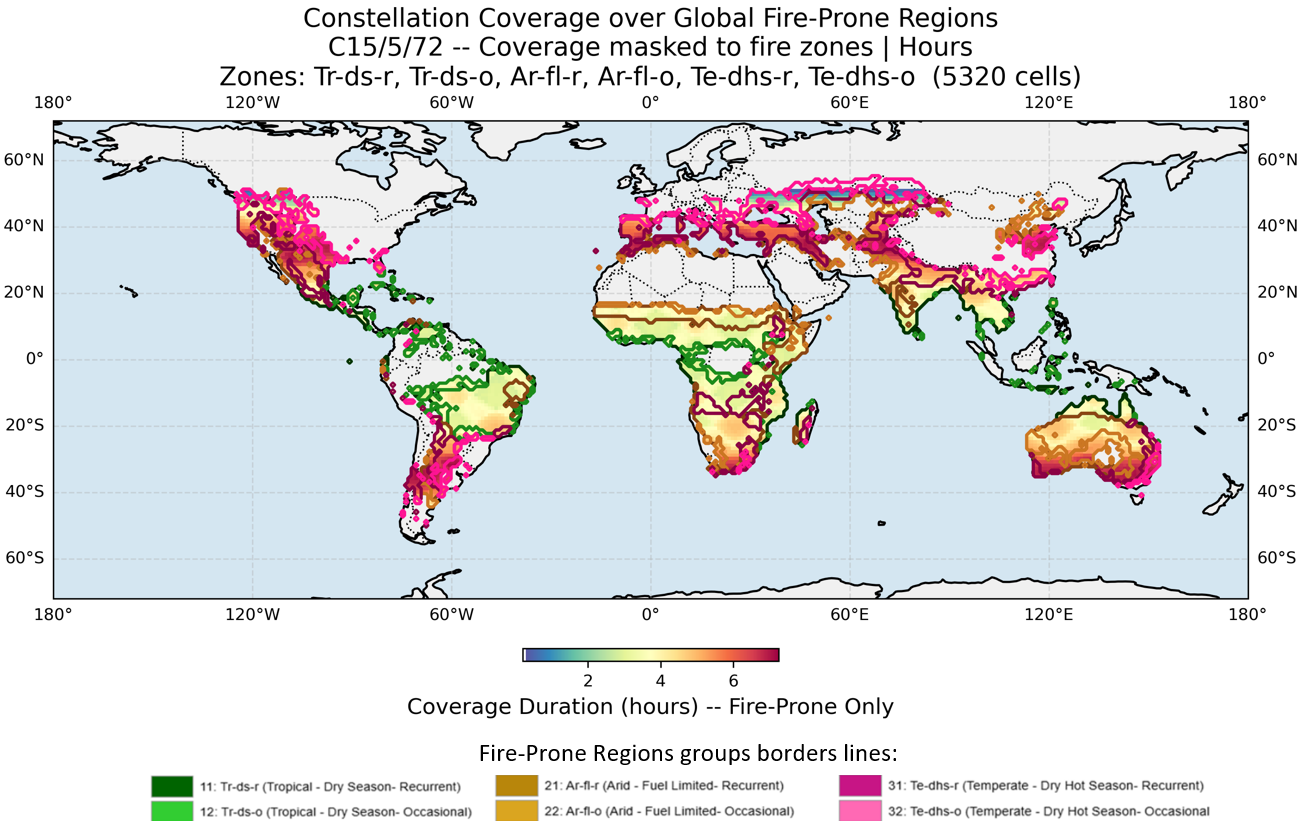
\includegraphics[width=1\linewidth]{images/c_zoom_global_FRP_recurrent_ocasional_Tcoverage_eta63.png}
    \caption{\footnotesize{Temporal coverage~$T_{\text{cov}}$ of the combined recurrent-and-occasional FPR mask for $\mathcal{C}_{\text{Zoom}}$ at the baseline $\eta = 65^{\circ}$.  The mask captures the operationally most relevant fire-prone regions worldwide; peak $T_{\text{cov}} \approx 6$--$7$\,h/day in the temperate belt ($\phi \approx \pm\,[30^{\circ}$--$45^{\circ}]$) and $T_{\text{cov}} > 3.5$\,h/day for other FPRs latitudes.  Boundaries-only and recurrent-only baseline maps are provided in Appendix~\ref{appendix-figures} (Figs.~\ref{fig:c_zoom_global_FRP_bondaries_Tcoverage_eta63}--\ref{fig:c_zoom_global_FRP_recurrent_Tcoverage_eta63}).}}
    \label{fig:c_zoom_global_FRP_recurrent_ocasional_Tcoverage_eta63}
\end{figure}


The temporal coverage maps for the remaining off-nadir configurations ($\eta = 45^{\circ}$, $30^{\circ}$, $15^{\circ}$) across all three FPR groups are provided in Appendix~\ref{appendix-figures}, Figs.~\ref{fig:c_zoom_global_FRP_boundaries_Tcoverage_eta45}--\ref{fig:c_zoom_global_FPR_recurrent_ocasional_Tcoverage_eta15}.


%%% 5c — FPR Coverage Statistics Summary
\subsubsection{Fire-Prone Region Coverage Statistics}
\label{sec:global_Domain_fire_prone_regions_statistics}

The bar-chart and scatter-plot breakdowns of the five performance variables across FPR groups and $\eta$ configurations are provided in Appendix~\ref{appendix-figures} (Figs.~\ref{fig:c_zoom_metrics_FPR_coverage_statistics}--\ref{fig:c_zoom_metrics_latitude_profile}).  Their results are consistent with the spatial maps above: the temperate-climate FPR group achieves the highest $T_{\text{cov}}$ and the shortest revisit times, while the constellation also operates over all other climate regions except boreal.  The latitude profile (Fig.~\ref{fig:c_zoom_metrics_latitude_profile}) is used in the following subsection to extract Portugal-specific metrics at $\phi = 40.02^{\circ}$\,N.

%%% ================================================================
%%% Phase 6 — Portugal Core Domain Performance
%%% ================================================================
\subsection{Portugal Core Domain Performance ($\mathcal{D}_{\text{core}}$)}
\label{sec:portugal_core_domain_metrics_derive_from_global_domain_results}

Reading the latitude profile (Fig.~\ref{fig:c_zoom_metrics_latitude_profile_not_norm} and Fig.~\ref{fig:c_zoom_metrics_latitude_profile}) at $\phi = 40.02^{\circ}$\,N at the constellation with baseline configuration ($\eta = 65^{\circ}$) generates the metrics for Portugal core-domain: \textbf{$T_{\text{cov}} \approx 6$\,h/day, $\bar{\eta} \approx 50^{\circ}$, $\Delta t_{\text{avg}} \approx 21$\,min, $\Delta t_{\max} \approx 34.67$\,min, and $\Delta t_{\min} \approx 12$\,min}.  These values satisfy the design targets \reqRef{R7}, \reqRef{R8}, \reqRef{R10}. The $t_{\mathrm{rev,P1}} \approx 33.41$ matches the inter-plane transit interval predicted in Section~\ref{sec:constellation_plane1}, while $\Delta t_{\min} \approx 12$\,min, arising from adjacent-plane overlap --- illustrated in Fig.~\ref{fig:obs_links_5planes},---  yields shorter revisit than originally anticipated from the single-plane design. \textbf{Leading to a better-than-expected average revisit time of $\Delta t_{\text{avg}} \approx 21$\,min, well below the design target of $t_{\text{revisit}} \approx 30$\,min.}  The $\bar{\eta} \approx 50^{\circ}$ at the core-domain latitude shown in Fig.~\ref{fig:c_zoom_avg_off_nadir} confirms that the constellation delivers the best observation geometry over Portugal, therefore, covering the full $\mathcal{D}_{\text{core}}$ defined in section \ref{sec_pt_space_domain}.

\subsection{Summary of Findings and Implications for the System Architecture}
\label{sec:zoom_layer_findings_summary}

The analysis presented in this section demonstrates that the $\mathcal{C}_{\text{Zoom}}$ constellation provides continuous temporal coverage over both the core domain~$\mathcal{D}_{\text{core}}$ and the global fire-prone regions, with revisit times that can reach sub-30-minute intervals not only over Portugal but across the temperate, tropical and arid FPR groups.  However, these performance levels are contingent on an effective sensor off-nadir capability of $\eta \approx 65^{\circ}$: the coverage maps and trade-off analysis (Table~\ref{tab:zoom_layer_configurations}) show that reducing $\eta$ rapidly degrades temporal resolution and demands a substantially larger constellation. Under constrained small satellite volumes, high spatial resolution sensor have narrow Field of View (FOV), exploiting the full geometric access envelope therefore requires the Zoom-layer instrument to be \emph{aimable}, capable of rapidly steering its FOV toward a designated target within the observation-link window.  This, in turn, implies a cueing mechanism that delivers timely fire-event information to the Zoom-layer spacecraft so that its sensor can be pointed in the correct direction before the access window closes.

A second finding emerges from the global pass-count and temporal-coverage maps (Figs.~\ref{fig:C_zoom_global_number_passes} and~\ref{fig:c_zoom_global_Tcovera_eta63}): the latitude band $\phi \approx \pm\,30^{\circ}$ concentrates the highest pass density and the peak $T_{\text{cov}}$, making it the geometrically optimal region for an inter-layer --- satellite-satellite or satellite-ground staiton ---  communication relay.  Taken together, these two results, the need for a cueing signal and the existence of a preferred relay latitude, define the functional requirements for a complementary constellation layer that can detect fire events at broad scale, relay the information to the Zoom layer, and enable targeted high-resolution observation.  The architecture that fulfils these requirements is proposed in the following section.


\section{Proposed Architecture: Watcher--Zoom ``Tip-and-Cue'' Concept}
\label{sec:proposed_architecture}

The preceding section established that $\mathcal{C}_{\text{Zoom}}$ can deliver sub-30-minute revisit with $\text{GSD} \approx 6$\,m/pixel over the core domain and global fire-prone regions, provided the sensor exploits an effective off-nadir envelope of $\eta \approx 65^{\circ}$.  Under small-satellite volume constraints, a high-spatial-resolution instrument has a narrow instantaneous FOV; therefore the Zoom-layer sensor must be \emph{aimable}, steered toward each fire target within the observation-link window.  This demands a cueing signal that arrives \emph{before} the access window closes.

In systems engineering, this cooperative multi-sensor strategy is known as a \emph{tip-and-cue} architecture (Fig.~\ref{fig:tip-and-cue_example}): each layer contributes a unique capability, one provides fast, coarse detection while the other delivers high-resolution confirmation.Their combination yields temporo-spatial fidelity unattainable by either layer alone~\cite{_architecture_tipcue}. 

Section~\ref{sec:geolayer_candidate_architecture} identified the existing geostationary fire-detection constellation composing the FIRMS dataset (Table~\ref{tab:geo_satellites}, Fig.~\ref{fig:firms_geostationary_sats}) as a candidate constellation $\mathcal{C}_{\text{Watcher}}$: five geostationary platforms (GOES-16/18, Meteosat-9/11, Himawari-8/9) that together cover Earth's full disk with a temporal resolution $\Delta t_{\text{Watcher}} \approx 10$--$15$\,min and a spatial resolution $\Delta s_{\text{Watcher}} \approx 2$--$3$\,km/pixel.

Figure~\ref{fig:watcher_zoom_3D_concept} illustrates the two-layer geometry: the geostationary $\mathcal{C}_{\text{Watcher}}$ layer provides continuous full-disk fire surveillance, while the LEO $\mathcal{C}_{\text{Zoom}}$ layer orbits beneath it.  The operational chain is detailed in Figure~\ref{fig:proposed_watcher_zoom_concept} and proceeds as follows.  A Watcher satellite $S_{\text{Watcher},i}$ detects fire activity and produces a coarse active-fire pixel (CAFPx) in its image $\mathcal{I}(S_{\text{Watcher},i})$, with $\Delta s_{\text{Watcher}} \approx 2$--$3$\,km/pixel and $\Delta t_{\text{Watcher}} \approx 10$--$15$\,min.  This detection is downlinked to a ground station via communication link~$\mathcal{L}_1$.  The ground segment relays the fire-alert message through link~$\mathcal{L}_2$ to a communication layer $\mathcal{C}_{\text{Comm}}$ (to be defined), which in turn transmits the cueing command via link~$\mathcal{L}_3$ to the Zoom-layer satellite $S_{\text{Zoom},k}$.  Upon reception, $S_{\text{Zoom},k}$ steers its dynamic boresight $\mathbf{b}_{k,\text{dynamic}}$ toward the CAFPx coordinates and acquires the fine active-fire pixel (FAFPx) image $\mathcal{I}(S_{\text{Zoom},k})$, with $\Delta s_{\text{Zoom}} \approx 6$\,m/pixel and $\Delta t_{\text{Zoom}} \lesssim 30$\,min (12--33\,min depending on inter-plane phasing).

\begin{figure}[H]
    \centering
    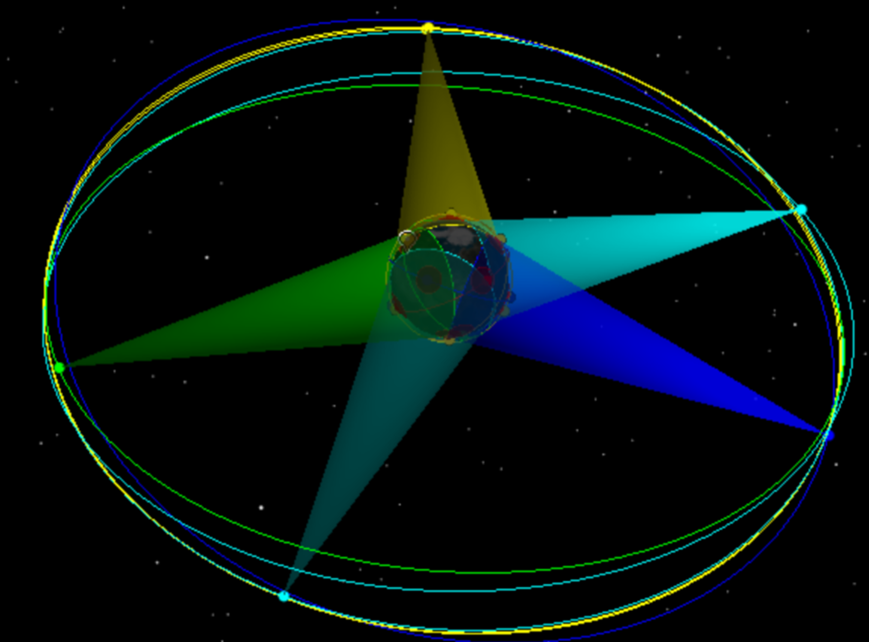
\includegraphics[width=0.5\linewidth]{images/watcher_zoom_3D_concept.png}
    \caption{\footnotesize{Watcher--Zoom two-layer constellation geometry. $\mathcal{C}_{\text{Watcher}}$ is defined as the five geostationary \emph{S-Watcher} satellites providing full-disk fire-detection coverage (FIRMS constellation, Table~\ref{tab:geo_satellites}). The $\mathcal{C}_{\text{Zoom}}$ LEO layer provides high-resolution active fire observation and is guided by the faster but coarser fire detection the geostationary Watcher layer.}}
    \label{fig:watcher_zoom_3D_concept}
\end{figure}

\begin{figure}[H]
    \centering
    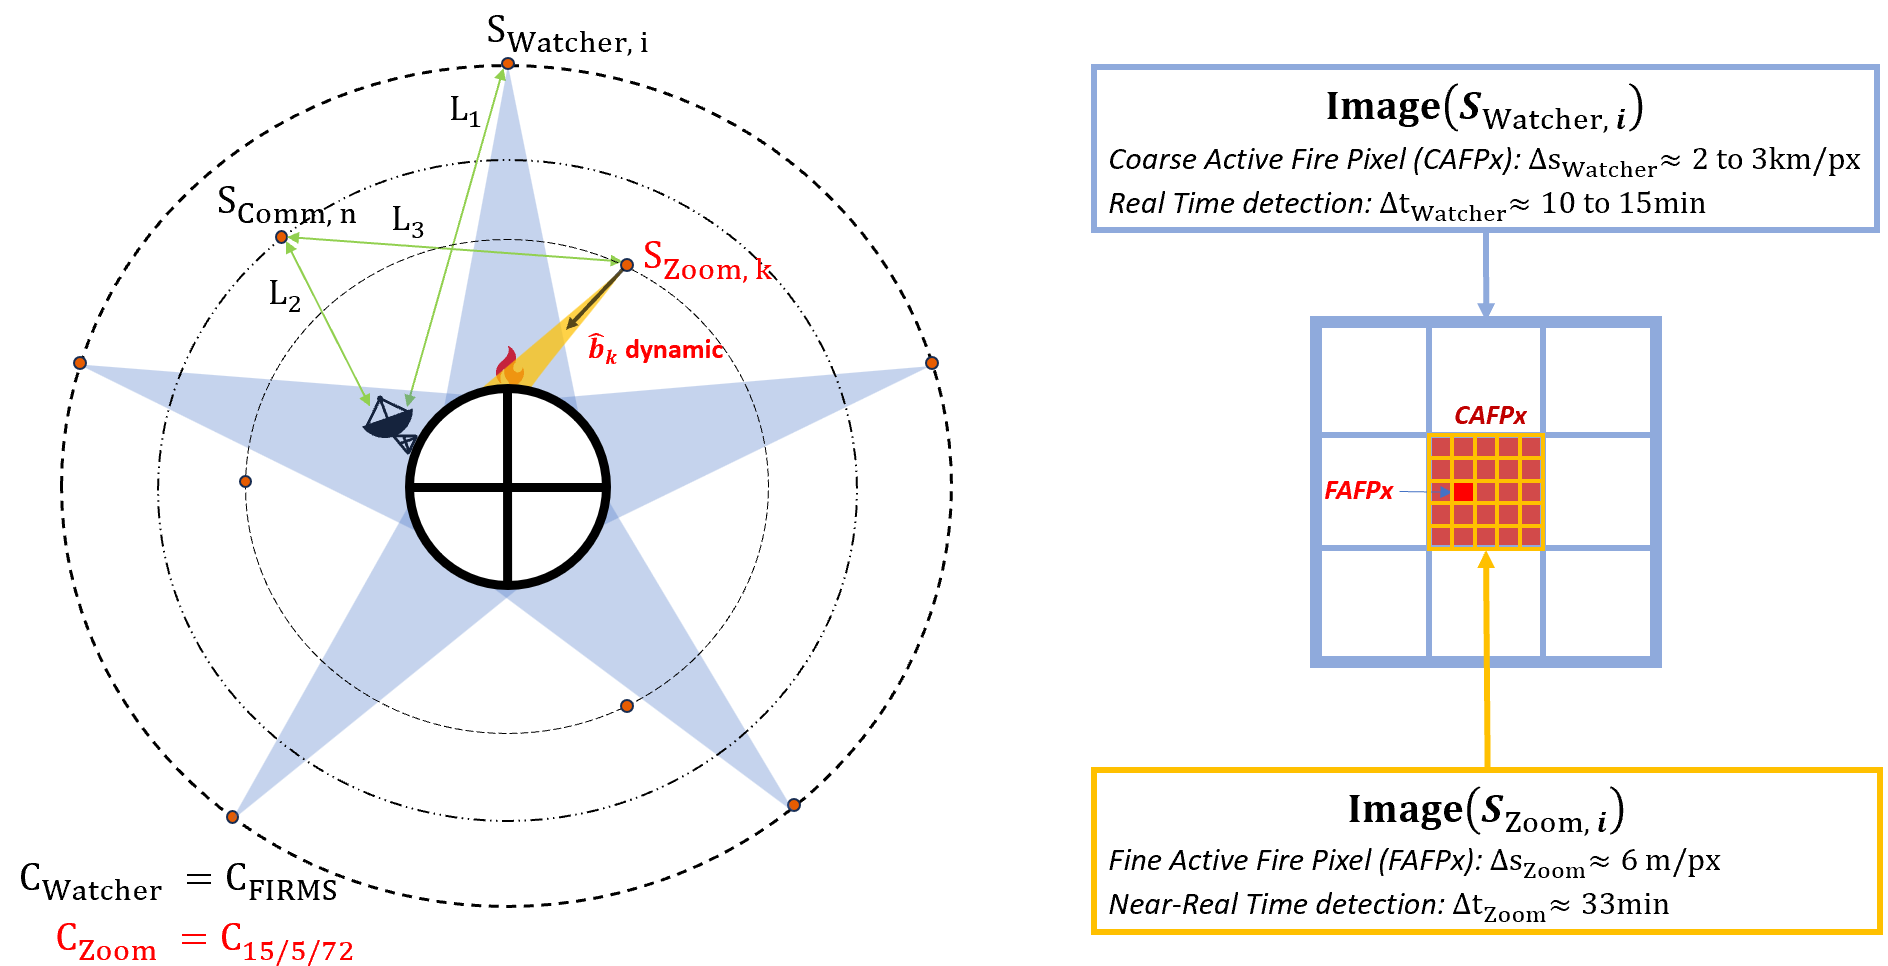
\includegraphics[width=1\linewidth]{images/proposed_watcher_zoom_concept.png}
    \caption{\footnotesize{Proposed Watcher--Zoom ``tip-and-cue'' operational concept.  \textbf{Left:} the $S_{\text{Watcher},i}$ layer detects an active fire and the alert propagates through the communication chain $\mathcal{L}_1 \to \mathcal{L}_2 \to \mathcal{L}_3$ to an $S_{\text{Zoom},k}$ satellite.  \textbf{Right:} Concept of alignment of the coarse active-fire pixel (CAFPX) from $\mathcal{I}(S_{\text{Watcher},i})$ ($\Delta s_{\text{Watcher}} \approx 1$--$3$\,km/pixel, $\Delta t_{\text{Watcher}} \approx 10$--$15$\,min) with the fine active-fire pixel (FAFPX) from $\mathcal{I}(S_{\text{Zoom},k})$ ($\Delta s_{\text{Zoom}} \approx 6$\,m/pixel, $\Delta t_{\text{Zoom}} \lesssim 30$\,min), demonstrating the tempo and spatial-resolution gain to detect active fire enabled by the fast cueing architecture.}}
    \label{fig:proposed_watcher_zoom_concept}
\end{figure}




% \begin{figure}[H]
%     \centering
%     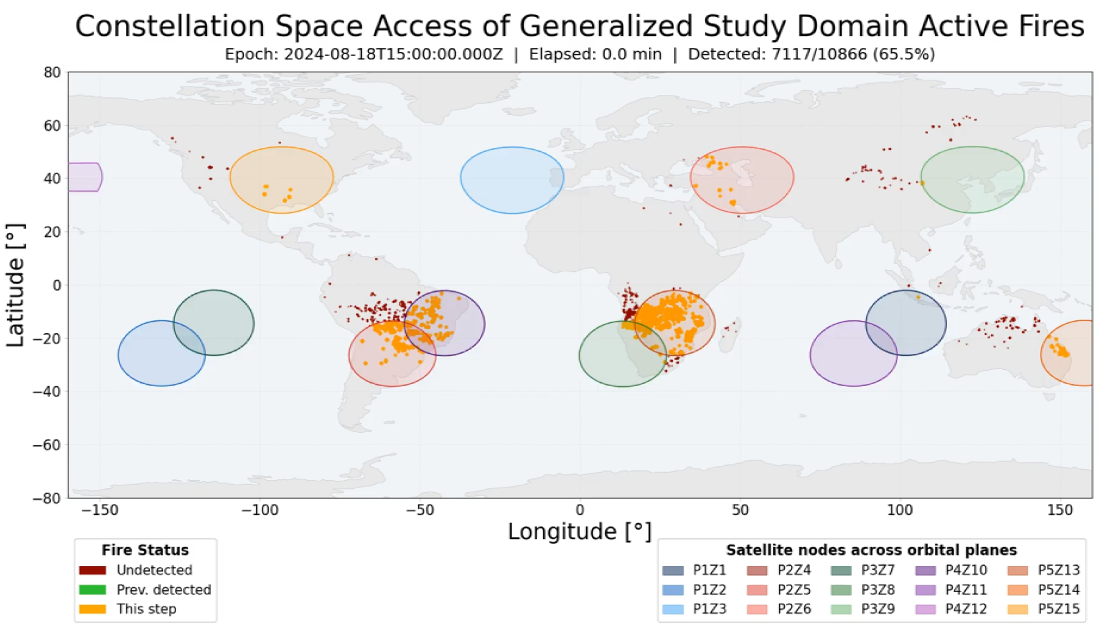
\includegraphics[width=1\linewidth]{images/concept_Watcher_Zoom_Space_access_simulation.png}
%     \caption{Enter Caption}
%     \label{fig:concept_Watcher_Zoom_Space_access_simulation}
% \end{figure}


\subsection{Constellation Architecture Initial Demonstration}
\label{sec:constellation_architecture_initial_demonstration}

With the Watcher--Zoom tip-and-cue architecture established, this subsection provides an initial demonstration of the concept through two complementary analyses: (i)~the observation-link capability of $\mathcal{C}_{\text{Zoom}}$ over real active-fire events, and (ii)~the feasibility of overlapping coarse and high-resolution fire imagery using existing satellite data as a proxy for the proposed system.

\subsubsection{Observation-Link Capability over Reference Fire Events}
\label{sec:concept_initial_observation_link_capability}

To evaluate the observation capacity of the $\mathcal{C}_{\text{Zoom}}$ layer over the $\mathcal{C}_{\text{Watcher}}$ geostationary fire-detection domain, the reference active-fire events $\Upsilon_{\text{fires}}$ defined in Section~\ref{sec:firms_dataset} are used.  These events, drawn from the FIRMS geostationary dataset, are populated over the global domain~$\mathcal{D}_{\text{global}}$, and each satellite of $\mathcal{C}_{\text{Zoom}}$ is propagated over this domain for a one-hour window.  Figure~\ref{fig:global_domain_active_fire_scan_onestep} shows the result: nearly 100\,\% of the concurrent active-fire events $\Upsilon_{\text{fires}}$ fall within the observation-link envelope at the baseline off-nadir angle $\eta_{\max} = 65^{\circ}$.

It must be noted that geometrical access does not imply a confirmed detection: actual fire observation requires a dedicated instrument with a defined swath, pointing mechanism, and collection schedule, all of which are outside the scope of this geometric study.  The simulation models the maximum effective field of view; in a higher-fidelity scenario the sensor would point within this detection envelope rather than covering it entirely.  Nonetheless, the simulator provides geometrically validated observation-link data over real fire events, establishing the foundation needed to support future instrument-level trade-offs---including sensor FOV, pointing range, swath width, image quality budgets, and onboard processing architectures such as in-orbit AI inference systems.

\begin{figure}[H]
    \centering
    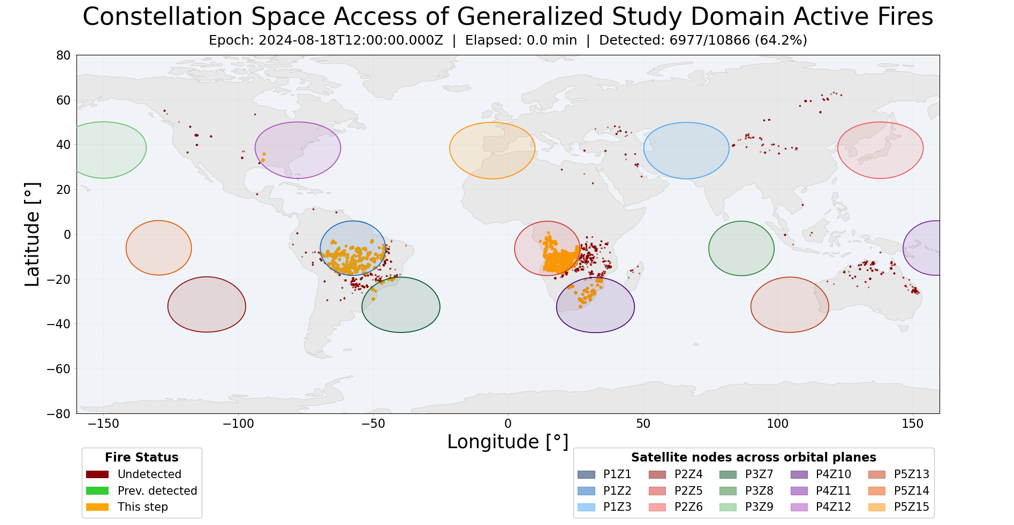
\includegraphics[width=0.75\linewidth]{images/global_domain_active_fire_scan_onestep.png}
    \caption{\footnotesize{Global-domain scan of the $\mathcal{C}_{\text{Zoom}}$ observation-link coverage over reference active-fire events~$\Upsilon_{\text{fires}}$.  Within a one-hour propagation window at $\eta_{\max} = 65^{\circ}$, nearly all concurrent global fire detections fall within the space-segment access envelope.  Geometrical access does not imply confirmed detection; the sensor footprint, pointing strategy, and collection schedule remain outside the scope of this geometric study.}}
    \label{fig:global_domain_active_fire_scan_onestep}
\end{figure}


\subsubsection{Coarse--Fine Image Overlap: Sentinel-2 as $\mathcal{C}_{\text{Zoom}}$ Proxy}
\label{sec:coarse_fine_image_overlap_demonstration}

The second demonstration evaluates the feasibility of overlapping a coarse active-fire pixel (CAFPx) from the $\mathcal{C}_{\text{Watcher}}$ layer with a high-resolution image from a LEO sensor.  Because the 15-satellite $\mathcal{C}_{\text{Zoom}}$ constellation is not yet deployed, the Sentinel-2 constellation is used as a proxy: Sentinel-2 operates at a similar LEO altitude and provides a fine active-fire pixel (FAFPx) at $\Delta s \approx 10$--$60$\,m/pixel, comparable in scale to the proposed $\mathcal{C}_{\text{Zoom}}$ GSD of $\approx 6$\,m/pixel.  The key difference is temporal resolution: Sentinel-2 revisits any given point with a five-day cadence, whereas the proposed constellation targets $\Delta t_{\text{Zoom}} \lesssim 30$\,min.

Figure~\ref{fig:proposed_watcher_zoom_initial_demonstration_w_Sentinel2_FIRMS} illustrates the concept: in the operational Watcher--Zoom architecture, $S_{\text{Watcher},i}$ provides the CAFPx that cues $S_{\text{Zoom},k}$; in this demonstration, the Sentinel-2 archive replaces $\mathcal{C}_{\text{Zoom}}$.  The algorithm proceeds as follows (Fig.~\ref{fig:fire_sanduich_Sentinel2_FIRMS_GOES_active_fire_algorithm}).  On a longitude--latitude--time domain, two Sentinel-2 archive images $\mathcal{I}(S_{\text{S2}}, t_1)$ and $\mathcal{I}(S_{\text{S2}}, t_2)$ are placed on the time axis, separated by the five-day revisit interval.  Simultaneously, the FIRMS $\mathcal{C}_{\text{Watcher}}$ constellation generates CAFPx detections every $\Delta t_{\text{Watcher}} \approx 10$--$15$\,min.  The matching criterion asks: \emph{does a Sentinel-2 image acquisition fall within $\pm\,15$\,min of a FIRMS CAFPx detection at the same location?} When this temporal coincidence is satisfied, the Sentinel-2 image has a high likelihood of containing active-fire pixels FAFPx that overlap the coarse FIRMS detection CAFPx, thereby demonstrating the tip-and-cue image-overlap concept.

\begin{figure}[H]
    \centering
    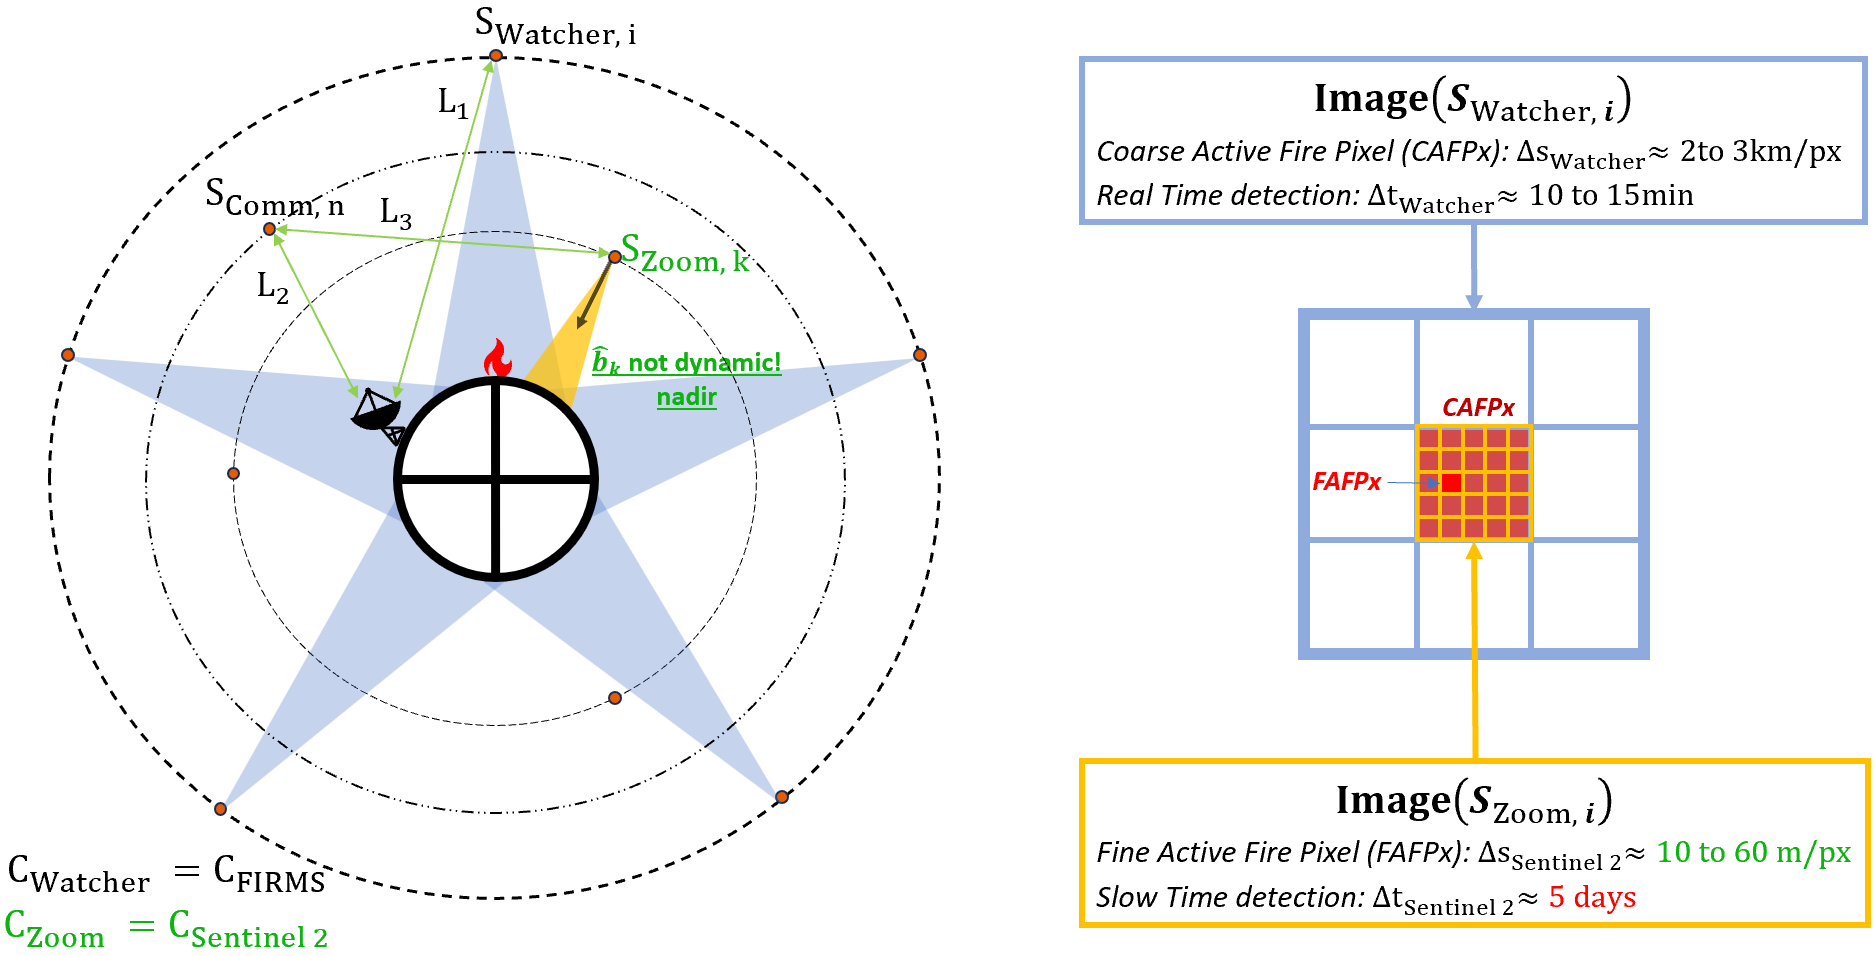
\includegraphics[width=1\linewidth]{images/proposed_watcher_zoom_initial_demonstration_w_Sentinel2_FIRMS.png}
    \caption{\footnotesize{Initial demonstration concept of the Watcher--Zoom image overlap using Sentinel-2 as a proxy for~$\mathcal{C}_{\text{Zoom}}$.  The $S_{\text{Watcher},i}$ layer (FIRMS geostationary constellation) provides the CAFPx detection ($\Delta s_{\text{Watcher}} \approx 2$--$3$\,km/pixel, $\Delta t_{\text{Watcher}} \approx 10$--$15$\,min), while the Sentinel-2 archive supplies the high-resolution counterpart (FAFPx, $\Delta s \approx 10$--$60$\,m/pixel) at a five-day revisit cadence.}}
    \label{fig:proposed_watcher_zoom_initial_demonstration_w_Sentinel2_FIRMS}
\end{figure}

\begin{figure}[H]
    \centering
    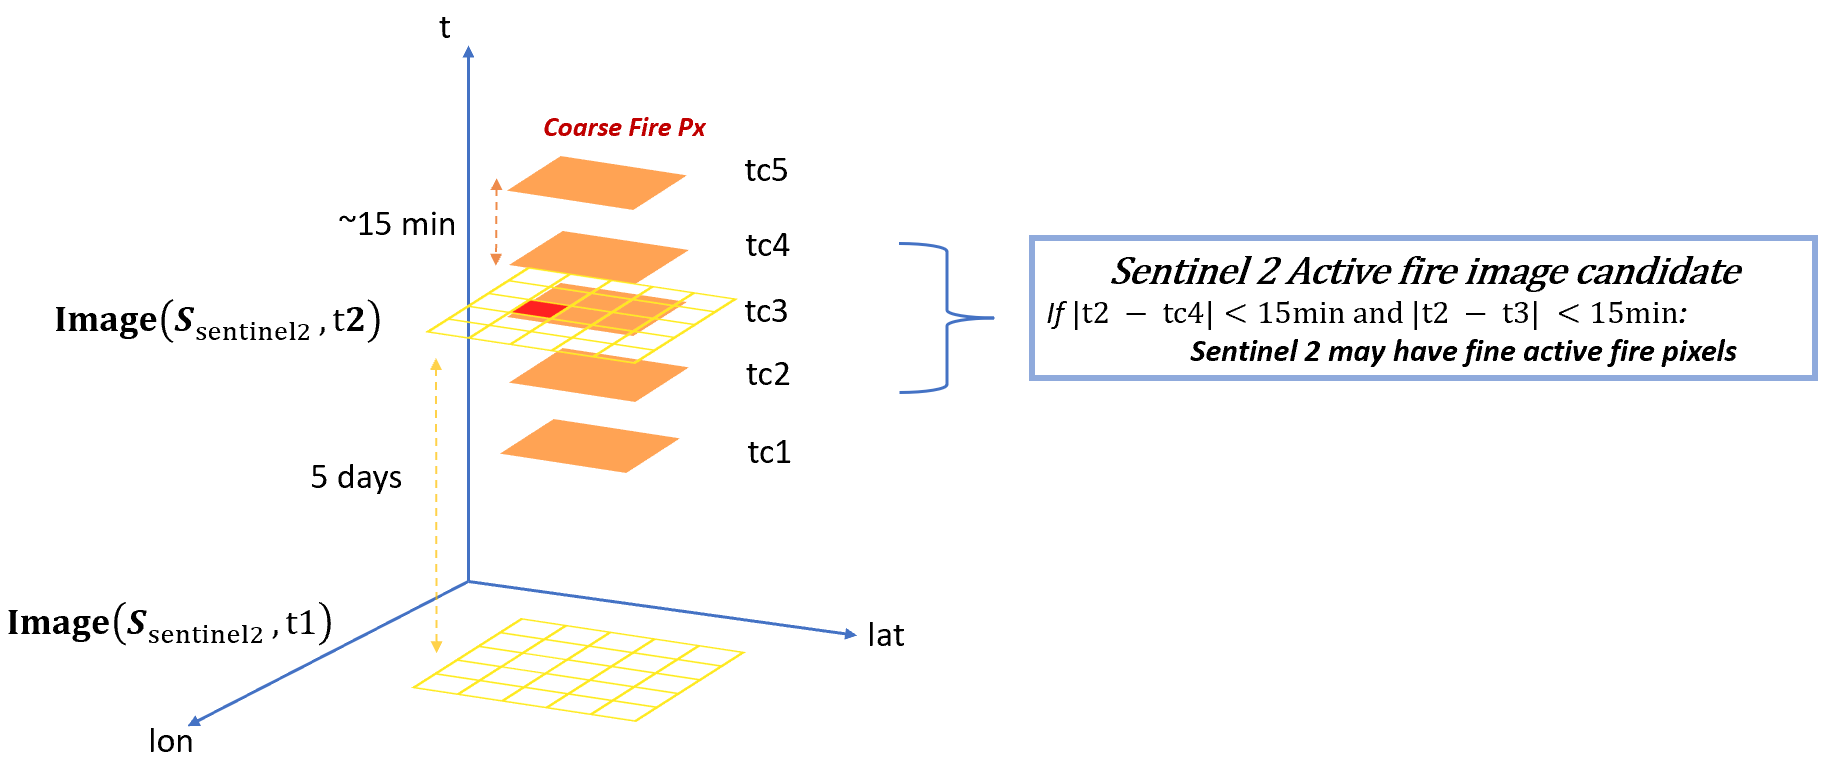
\includegraphics[width=0.8\linewidth]{images/fire_sanduich_Sentinel2_FIRMS_GOES_active_fire_algorithm.png}
    \caption{\footnotesize{Temporal-coincidence algorithm for the coarse--fine image overlap demonstration.  The longitude--latitude--time diagram shows Sentinel-2 archive images $\mathcal{I}(S_{\text{S2}}, t_1)$ and $\mathcal{I}(S_{\text{S2}}, t_2)$ on the time axis, together with the FIRMS $\mathcal{C}_{\text{Watcher}}$ CAFPx detections at $\Delta t_{\text{Watcher}} \approx 10$--$15$\,min cadence.  A match is declared when a Sentinel-2 acquisition falls within $\pm\,15$\,min of a FIRMS detection at the same location, indicating a high likelihood of active-fire pixels in the Sentinel-2 image.}}
    \label{fig:fire_sanduich_Sentinel2_FIRMS_GOES_active_fire_algorithm}
\end{figure}


Applying this temporal-coincidence scan over the full year 2024 using the Google Earth Engine Sentinel-2 archive, a total of 3062 active-fire images were identified globally (Fig.~\ref{fig:active_fire_dataset_global_2024_FIRMS_Sentinel2}).  This relatively small yield reflects the stringent five-day revisit of Sentinel-2: the probability of a temporal coincidence between a Sentinel-2 pass and a FIRMS detection within a 15-minute window is inherently low.  This scarcity underscores the need for a dedicated LEO constellation with sub-30-minute revisit to ensure systematic coarse--fine overlap.

\begin{figure}[H]
    \centering
    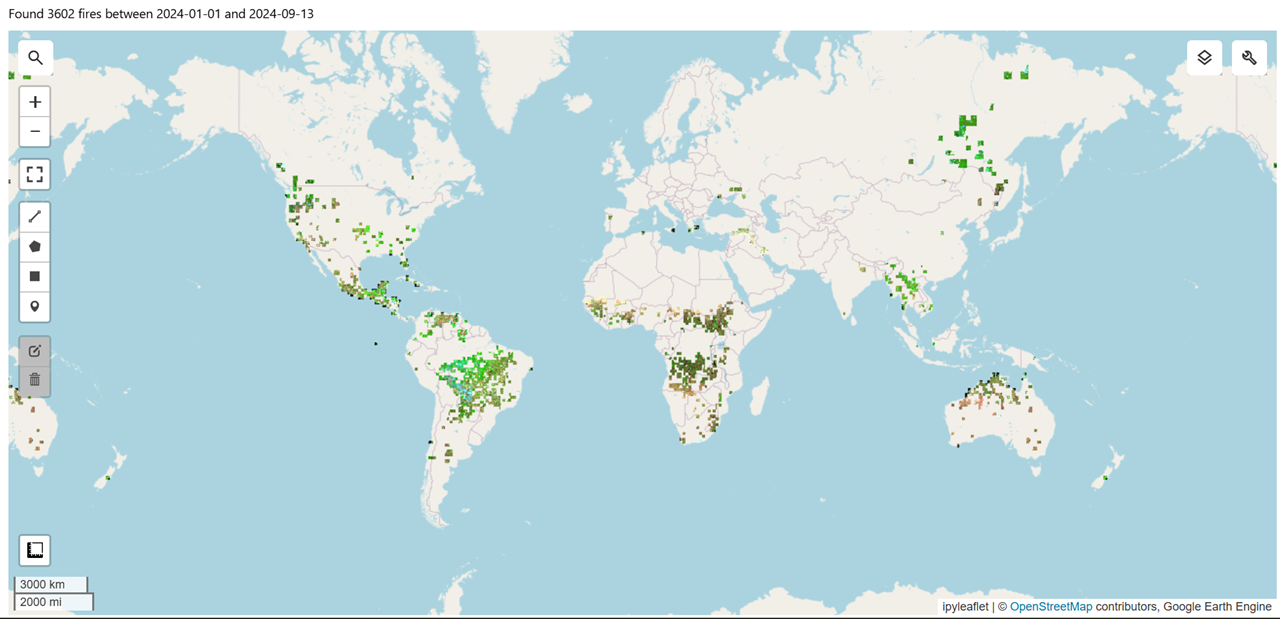
\includegraphics[width=0.8\linewidth]{images/active_fire_dataset_global_2024_FIRMS_Sentinel2.png}
    \caption{\footnotesize{Global map of the 3062 active-fire images identified in 2024 by the temporal-coincidence algorithm applied to the Sentinel-2 archive and FIRMS $\mathcal{C}_{\text{Watcher}}$ CAFPx dataset.  Each marker represents a Sentinel-2 acquisition that fell within $\pm\,15$\,min of a FIRMS geostationary fire detection, confirming coarse--fine image overlap at that location.}}
    \label{fig:active_fire_dataset_global_2024_FIRMS_Sentinel2}
\end{figure}

Two representative cases illustrate the overlap fidelity.  Figure~\ref{fig:portugal_Viseu_2024-08-16_fire_Watcher_Firms_Zoom_S2_fire_pixels} shows the only fire event captured over Portugal in 2024 by this method: a wildfire near Viseu (2024-08-16), close to the core-domain latitude $\phi \approx 40^{\circ}$\,N.  The Sentinel-2 image reveals a active fire event tt high resolution pixel level FAFPx, while the large blue pixels are the Fire Radiative Power gradient emmite by the fire($\sim\!2$\,km scale) represent the FIRMS CAFPx detections from $\mathcal{C}_{\text{Watcher}}$. Check equation \ref{eq:frp_operational} for more about FRP.  The two datasets are nearly co-located, confirming that the coarse Watcher-layer detection correctly flags the region where the high-resolution sensor observes active fire. Simulating the behaviour the tip-and-cue architecture is designed to exploit.

Figure~\ref{fig:australia_fire_2024-04-17_big} presents a second, larger-scale example: an Australian wildfire (2024-04-17) with a nearly continuous fire front extending $\sim\!37$\,km.  Fire radiative power in this event reaches $\sim\!1{,}000$\,MW, compared with $\sim\!297$\,MW for the Portuguese case, illustrating the dynamic range of fire intensity the system must accommodate.

Together, these two demonstrations confirm that: (i)~the $\mathcal{C}_{\text{Zoom}}$ observation-link geometry covers nearly all global active-fire events within a one-hour window, and (ii)~real satellite data validate that a coarse geostationary detection can reliably flag the location where a high-resolution LEO sensor observes active fire.  What the current demonstrations lack is the dynamic pointing capability .  Realising the operational architecture therefore requires the communication layer~$\mathcal{C}_{\text{Comm}}$ to relay cueing commands from the Watcher layer to the Zoom layer in near-real time, a component addressed in subsequent system-level design.

\begin{figure}[H]
    \centering
    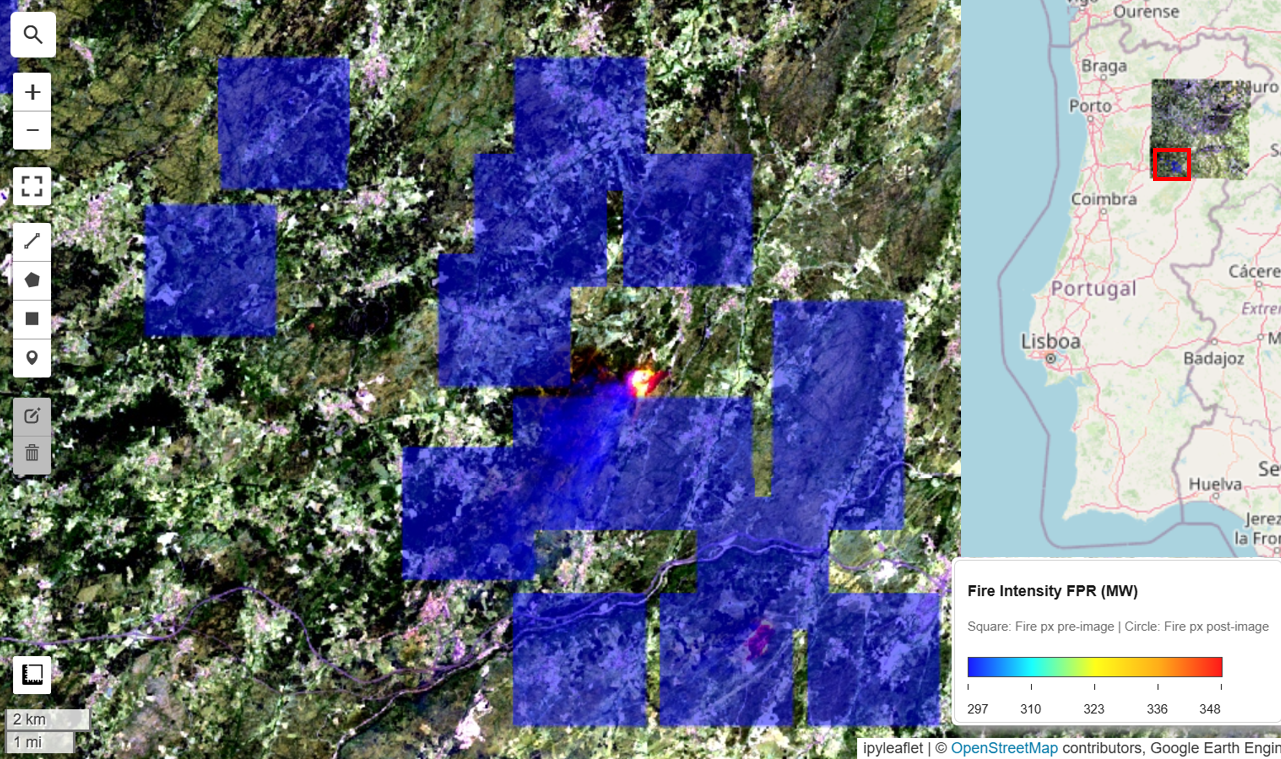
\includegraphics[width=0.9\linewidth]{images/portugal_Viseu_2024-08-16_fire_Watcher_Firms_Zoom_S2_fire_pixels.png}
    \caption{\footnotesize{Coarse--fine image overlap for the Viseu (Portugal) wildfire, 2024-08-16.  The Sentinel-2 per-pixel fire-intensity gradient (FAFPx, $\Delta s \approx 10$--$60$\,m/pixel) is overlaid with the FIRMS $\mathcal{C}_{\text{Watcher}}$ coarse active-fire pixels (CAFPx, $\Delta s \approx 2$\,km/pixel, blue).  The near co-location of the two datasets demonstrates the feasibility of the Watcher-layer cueing concept: the CAFPx correctly flags the region where high-resolution active fire is observed.  Fire radiative power $\approx 297$\,MW.}}
    \label{fig:portugal_Viseu_2024-08-16_fire_Watcher_Firms_Zoom_S2_fire_pixels}
\end{figure}

\begin{figure}[H]
    \centering
    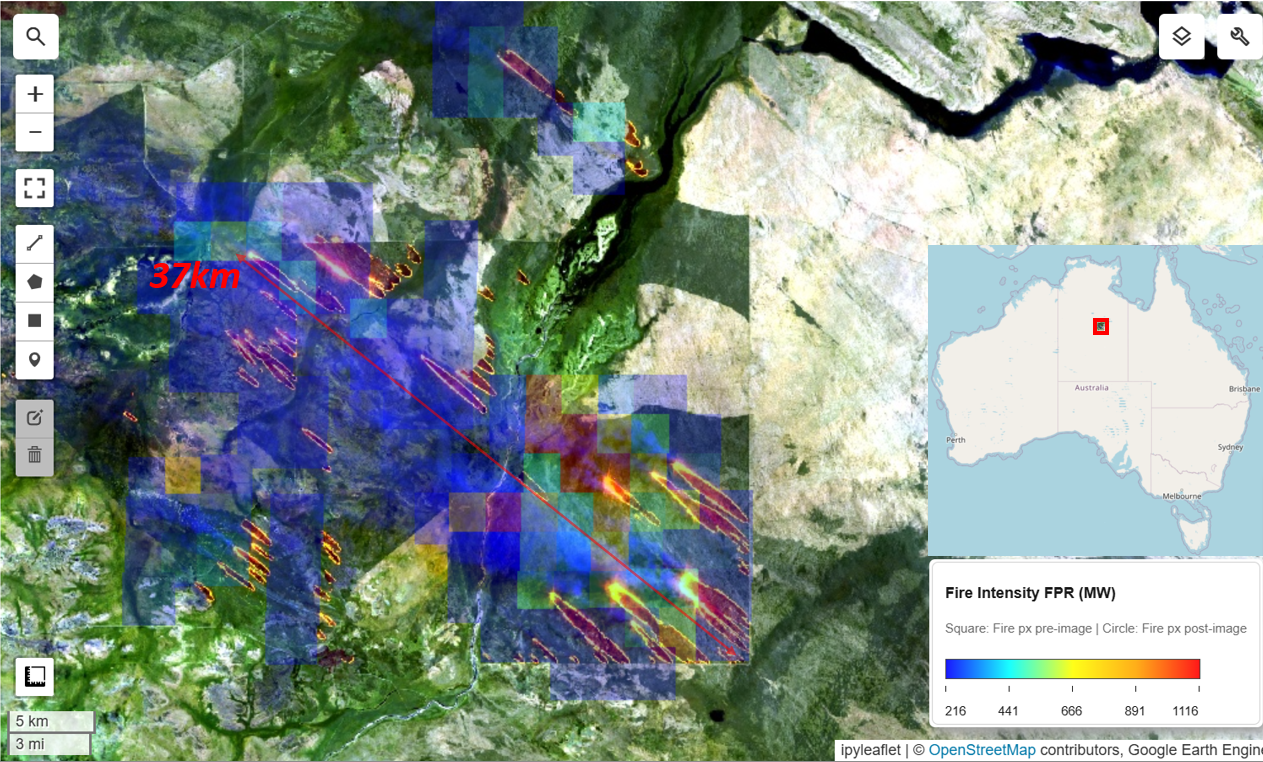
\includegraphics[width=0.9\linewidth]{images/australia_fire_2024-04-17_big.png}
    \caption{\footnotesize{Coarse--fine image overlap for an Australian wildfire, 2024-04-17.  The fire front extends $\sim\!37$\,km with fire radiative power reaching $\sim\!1{,}000$\,MW.  As in the Portuguese case, the FIRMS CAFPx detections (blue, $\Delta s \approx 2$\,km/pixel) align with the Sentinel-2 FAFPx active-fire pixels, confirming the tip-and-cue overlap concept at a substantially larger fire scale.}}
    \label{fig:australia_fire_2024-04-17_big}
\end{figure}



% \section{Conceptual Payload \& Communications
% Requirements}\label{92-conceptual-payload--communications-requirements}
% \fxwarning{Write brief section on payload and communication limitations: top-level imaging payload requirements and communication constraints between Zoom layer and ground/AGIF system. Keep concise---detailed sizing is future work.}

% \section{Concept of Operations
% (CONOPS)}\label{93-concept-of-operations-conops}
% \fxwarning{Write CONOPS narrative: day-in-the-life scenario from fire detection in Portugal to data delivery to AGIF fire-combat system. Add architecture diagram connecting Watcher layer $\to$ Zoom layer $\to$ ground segment $\to$ AGIF.}
